%!TEX encoding = UTF-8 Unicode


\immediate\write18{makeindex \jobname.nlo -s nomencl.ist -o \jobname.nls}
\immediate\write18{bibtex \jobname.aux}
\documentclass[a4paper,fleqn,12pt,headsepline]{scrartcl}

% Mit \usepackage bindet man Sammlungen nützlicher Befehle,
% sog. Pakete ein. Das graphicx-Paket stellt z.B. einen Befehl
% \includegraphics zur Verfügung, mit dem man (bei Verwendung von
% PDFLaTeX) Grafiken im PDF-, PNG- oder JPG-Format einbinden kann.
%
\usepackage{graphicx}

% Umlaute und sonstige Sonderzeichen als UTF-8 direkt eingeben
%\UseRawInputEncoding
\usepackage[utf8]{inputenc}

% Sprachpaket „reformierte deutsche Rechtschreibung“ einbinden
% (u.a. für Trennungen)
\usepackage[ngerman]{babel}	% Für Englische Berichte ausqwählen und auskommentieren
%\usepackage[english]{babel} 		% Für Englische Berichte ausqwählen und auskommentieren
%\usepackage[french]{babel}

% Zeichensätze und Zeichensatzkodierung auswählen
%
% Unten sind verschiedene Möglichkeiten aufgeführt, aber nur eine
% wird tatsächlich verwendet. Die anderen sind „auskommentiert“;
% um diese auszuprobieren, genügt es, Kommentarzeichen zu verschieben.
%
\usepackage[T1]{fontenc}
%
%\usepackage{fix-cm} % Standard-Schriftfamilie “Computer Modern” in einer flexibleren Variante verwenden
\usepackage{lmodern} % Schriftfamilie „Latin Modern“ (Erweiterung von „Computer Modern“) verwenden
%\usepackage{droid} % Schriftfamilie „Droid“ verwenden
%\usepackage{times} % „Times New Roman” als Serifenschrift verwenden
%\usepackage{librebaskerville} % „Libre Baskerville” als Serifenschrift verwenden
%\usepackage{libertine} % „Linux Libertine” als Serifenschrift verwenden
%\usepackage{fourier} % „Utopia Regular” als Serifenschrift verwenden
%\usepackage{fouriernc} % „New Century Schoolbook” als Serifenschrift verwenden
%\usepackage{tgschola} % „TeX Gyre Schola” als Serifenschrift verwenden
%\usepackage[scaled=0.95]{helvet} % leicht verkleinerte „Helvetica“ als Sans-Serif-Schrift verwenden
%
% Sans-Serif-Schrift als Standardschrift benutzen
%\renewcommand*\familydefault{\sfdefault}

% Wenn man Anführungszeichen unten und oben nicht von Hand eingeben
% will oder kann (z.B. „Test“), ermöglicht das csquotes-Paket u.a.,
% stattdessen \enquote{Test} zu schreiben.
%
%\usepackage[babel,german=quotes]{csquotes}	% Nur für deutsche berichte einkommentieren
% 

% Das float-Paket stellt erweiterte Möglichkeiten zur Plazierung von
% Abbildungen und sonstiger „gleitender“ Inhalte zur Verfügung.
%
\usepackage{float}

% Bilder mit „Bild“ anstatt mit „Abbildung“ bezeichnen
%\renewcaptionname{ngerman}\figurename{Bild} % für deutsche Berichte inkommentiern nur 
%\figurename{Fig:}  		% nur für englische Verichte einmkommentieren 

% Das picins-Paket stellt Befehle zur Verfügung, Bilder in den Text
% zu integrieren und umfließen zu lassen.
%
%\usepackage{picins}

% Bilder, Tabellen usw. sind in LaTeX normalerweise „gleitend“,
% d.h., sie stehen nicht an einer bestimmten Stelle im Text, sondern
% z.B. oben auf der Seite. Wenn man Bilder usw. nicht gleiten läßt,
% sondern sie fest mit dem Text verbindet, ermöglicht dieses Paket,
% ihre Beschriftung (caption) dennoch im Abbildungsverzeichnis
% erscheinen zu lassen und darauf zu verweisen.
%
% Die hier verwendete KOMA-Version scrartlc des Artikel-Formats
% enthält bereits die in diesem Paket enthaltenen Befehle. Sie
% benötigen es daher nur, wenn Sie das Standard-Artikel-Format
% article verwenden.
% 
%\usepackage{capt-of}

% Paket für mehrseitige Tabellen
%\usepackage{longtable}

% Paket für Seitenrandabstände und Einstellung für Seitenränder
\usepackage{geometry}
\geometry{left=3.5cm, right=2cm, top=2.5cm, bottom=2cm}

% Paket für Kästchen mit Spezialeffekten (z.B. Schatten)
%\usepackage{fancybox}

% bricht lange URLs „schön“ um
\usepackage[hyphens,obeyspaces,spaces]{url}

% Paket für Textfarben
\usepackage{color}

% Zusätzliche mathematische Symbole importieren
\usepackage{amsmath}
\usepackage{amssymb}

% erzeugt Inhaltsverzeichnis mit Querverweisen zu den Kapiteln (PDF Version)
\usepackage[bookmarksnumbered,hyperfootnotes=false]{hyperref} 
\hypersetup{colorlinks,citecolor=black,linkcolor=black,urlcolor=black}

% neue Kopfzeilen mit dem fancyhdr-Paket erzeugen
\usepackage{fancyhdr} % Paket laden
\pagestyle{fancy} % eigener Seitenstil
\fancyhf{} % alle Kopf- und Fußzeilenfelder bereinigen
\fancyhead[L]{\nouppercase{\leftmark}} % Kopfzeile links
\fancyhead[C]{} % zentrierte Kopfzeile
\fancyhead[R]{\thepage} % Kopfzeile rechts
\renewcommand{\headrulewidth}{0.4pt} % obere Trennlinie

% Festlegung der Art der Zitierung auf die Havard-Methode: Abkürzung Autor + Jahr.
% Dieser Befehl gehört zum natbib-Paket.
%
\usepackage[square,sort,comma,numbers]{natbib}
\bibliographystyle{plainnat}

% keine Einrückung am Anfang eines Absatzes,
% stattdessen vertikal etwas Platz lassen
%
\usepackage{parskip}

% Paket zur Erweiterung der Tabellen-Befehle (tabular, array)
%\usepackage{array}

% Dieser Befehl würde den zusätzlichen Zwischenraum abschalten,
% den LaTeX normalerweise nach einem Punkt einfügt.
%\frenchspacing

% Paket für Zeilenabstand einbinden
%\usepackage{setspace}
% Dieser Befehl würde den Zeilenabstand auf „1,5“ einstellen
%\onehalfspacing

% Paket für Listings (z.B. Computerprogramme)
\usepackage{listings}
\usepackage{xcolor}
%
% Einstellungen für C-Quelltexte
%\lstset{numbers=left,
%        numberstyle=\tiny,
%        numbersep=5pt,
%        keywordstyle=\color{black}\bfseries,
%        stringstyle=\ttfamily,
%        showstringspaces=false,
%        basicstyle=\footnotesize,
%        captionpos=b}
%\lstset{language=c}
%
% Einstellungen für LaTeX-Quelltexte
%\lstset{basicstyle=\ttfamily, language=text}


%%%%%%%DEFAULT-LANGAUGE%%%%%%%%%%%%%%%%%%
% 
\lstset{basicstyle=\color{blendedblue},
        language=C,
        captionpos=b,
        gobble=4,
        xleftmargin=1em,
        columns=fullflexible,
        moredelim=**[is][\color{red}]{¡}{¿}
      }

%%%%%%%%%%%%%%%%%%%%%%%%%%%%%%%%%%%%%%%
%%%%%%%PYTHON-LANGAUGE%%%%%%%%%%%%%%%%%%


% Default fixed font does not support bold face
\DeclareFixedFont{\ttb}{T1}{txtt}{bx}{n}{12} % for bold
\DeclareFixedFont{\ttm}{T1}{txtt}{m}{n}{12}  % for normal

% Custom colors
\usepackage{color}
\definecolor{blendedblue}{rgb}{0.2,0.2,0.7}
\definecolor{deepblue}{rgb}{0,0,0.5}
\definecolor{deepred}{rgb}{0.6,0,0}
\definecolor{deepgreen}{rgb}{0,0.5,0}

\lstset{basicstyle=\color{blendedblue},
        language=C,
        captionpos=b,
        gobble=4,
        xleftmargin=1em,
        columns=fullflexible,
        moredelim=**[is][\color{red}]{¡}{¿}}


% Python style for highlighting
\newcommand\pythonstyle{\lstset{
language=Python,
basicstyle=\ttfamily,
morekeywords={self},              % Add keywords here
keywordstyle=\ttb\color{deepblue}\small,
emph={MyClass,__init__},          % Custom highlighting
emphstyle=\ttb\color{deepred}\small,    % Custom highlighting style
stringstyle=\color{deepgreen}\small,
frame=shadowbox,                         % Any extra options here
showstringspaces=false,
columns=fullflexible,
breaklines = true,
}
}


% Python environment
\lstnewenvironment{python}[1][]
{
\pythonstyle
\lstset{#1}
}
{}


% Python for external files
\newcommand\pythonexternal[2][]{{
\pythonstyle
\lstinputlisting[#1]{#2}}}

% Python for inline
\newcommand\myPython[1]{{\pythonstyle\lstinline!#1!}}
%\newcommand\pythoninline[1]{{\pythonstyle\lstinline!#1!}}
%\newcommand\mylstinline[1]{{\pythonstyle\lstinline!#1!}}



%%%%%%%%%%%%%%%%%%%%%%%%%%%%%%%%%%%%%%%
%FIXME: bash environment doesn't work
%%%%%%%BASH-LANGAUGE%%%%%%%%%%%%%%%%%%
%Quelle: https://tex.stackexchange.com/questions/84185/displaying-linux-commands-in-latex
%\usepackage{pythontex}
%\usepackage{fancyvrb}
%\setpygmentspygopt{bash}{style=default} %Set syntax highlighting style
%\setpygmentsfv{xleftmargin=4ex} %Pass fancyvrb options, in this case, left margin

\newcommand\bashstyle{\lstset{
language=bash,
basicstyle=\ttfamily,
morekeywords={self},              % Add keywords here
keywordstyle=\ttb\color{deepblue}\small,
emph={MyClass,__init__},          % Custom highlighting
emphstyle=\ttb\color{deepred}\small,    % Custom highlighting style
stringstyle=\color{deepgreen}\small,
frame=shadowbox,                         % Any extra options here
showstringspaces=false,
columns=fullflexible,
breaklines = true,
% basicstyle=\ttfamily,
% % morekeywords={self},              % Add keywords here
% % keywordstyle=\ttb\color{deepred}\small,
% % emph={MyClass,__init__},          % Custom highlighting
% % emphstyle=\ttb\color{deepred}\small,    % Custom highlighting style
% % stringstyle=\color{deepred}\small,
% % frame=shadowbox,                         % Any extra options here
% % showstringspaces=false,
% columns=fullflexible,
% breaklines = true,
}
}

\lstnewenvironment{bash}[1][]
{
\bashstyle
\lstset{#1}
}
{}


%%%%%%%%%%%%%%%%%%%%%%%%%%%%%%%%%%%%%%%



\usepackage{siunitx}


% Nomenklatur
%
% Paket einbinden
\usepackage{nomencl}
%
% Befehl „\nomenclature” alternativ als „\abk“ zur Verfügung stellen
\let\abk\nomenclature
%
% Deutsche Überschrift für Nomenklaturverzeichnis
\renewcommand{\nomname}{Nomenklatur} % nur für deutsche Berichte 
%
% Nomenklaturverzeichnis gestalten
% Raum, der den Abkürzungen zur Verfügung steht = 0.2 der Gesamtbreite
\setlength{\nomlabelwidth}{0.2\hsize}
% Zeilenabstände verkleinern
\setlength{\nomitemsep}{-\parsep}
\makenomenclature
% Erstellen von Unterteilungen in der Nomenklatur
\RequirePackage{ifthen}
\renewcommand{\nomgroup}[1]{%
  \ifthenelse{\equal{#1}{A}}{\item[\textbf{Abkürzungen}]\vspace*{1cm}}{%
    \ifthenelse{\equal{#1}{S}}{%
      \item[\textbf{Symbole}]\vspace*{1cm}}{}%
  }%
}


% Benutzte in Überschrift die gleiche Schriftart und Farbe wie im Text
\setkomafont{disposition}{\normalcolor\bfseries}

% Maßeinheit für picture-Grafiken
\setlength{\unitlength}{1cm}

%
% fuer Stichwortverzeichnis
%\usepackage{makeidx}
% Stichwortverzeichnis erstellen
%\makeindex
%\renewcommand{\indexname}{Stichwortverzeichnis} % nur für deutsche Berichte 

%%%%%%%%%%%%%%%
% pgfplots und tikz
\usepackage{tikz}
\usepackage{pgfplots}

\usetikzlibrary{patterns}
\usetikzlibrary{datavisualization}
\usetikzlibrary{arrows}

\usepackage{textcomp}
\usepackage{gensymb}
\usepackage{booktabs}
\usepackage{longtable}
\usepackage{multirow}
\usepackage[toc,page]{appendix} % für englische Berichte

%\usepackage{minted}


% Bildnummern aus Nummer des Abschnitts und laufender Nummer zusammensetzen
%
% Bei Verwendung eines Bericht-Formats (s.o.) geschieht dies
% automatisch mit der Kapitelnummer (\chapter – eine Ebene oberhalb
% von \section). Für das Artikel-Format machen wir es hier manuell.
%
\renewcommand{\thefigure}{\arabic{section}.\arabic{figure}}
\makeatletter\@addtoreset{figure}{section}\makeatother

% Gleichungsnummern aus Nummer des Abschnitts und laufender Nummer zusammensetzen
\renewcommand{\theequation}{\arabic{section}.\arabic{equation}}
\makeatletter\@addtoreset{equation}{section}\makeatother

% Tabellennummern aus Nummer des Abschnitts und laufender Nummer zusammensetzen
\renewcommand{\thetable}{\arabic{section}.\arabic{table}}
\makeatletter\@addtoreset{table}{section}\makeatother



% auf römische Seitenzahlen umschalten
%\pagenumbering{Roman}

% Mit \input wird eine selbst erstellte .tex-Datei eingebunden.
%
% „trennung.tex“ enthält ein (selbst erstelltes) Verzeichnis mit
% Trennhilfen für häufige Wörter, deren Silbentrennung von der
% Automatik nicht korrekt erkannt wird.
%
%hier müssen alle Wörter rein, welche Latex von sich auch nicht korrekt trennt bzw. bei denen man die genaue Trennung vorgeben möchte
\hyphenation{
Film-pro-du-zen-ten
Lux-em-burg
Soft-ware-bau-steins
zeit-in-ten-siv
wis-sen-schaft-li-chen
ent-spre-chend
}

% Mit \newcommand definieren wir einen neuen Befehl.
% Die 1 in eckigen Klammern bedeutet, daß der Befehl einen Parameter
% (bei Verwendung in geschweiften Klammern zu setzen) akzeptiert.
% Mit #1 nehmen wir auf diesen Parameter bezug.
%
% Der Befehl bewirkt, daß der Parameter in Sans-Serif-Schrift gesetzt wird.
%
% Beispiel für die Verwendung des Befehls: \file{hauptdatei.tex}
%
% Man könnte natürlich auch direkt \textsf{hauptdatei.tex} schreiben.
% Der neue Befehl hat aber den Vorteil, daß er markiert, was wir meinen
% und nicht, wie es aussehen soll. Konkret: Wenn wir uns im Nachhinein
% dafür entscheiden, Dateinamen doch nicht in Sans-Serif-Schrift, sondern
% z.B. kursiv zu setzen, muß dafür nur die Befehlsdefinition geändert werden
% – und nicht jede einzelne Stelle, an der der Befehl verwendet wird.
%
\newcommand{\file}[1]{\textsf{#1}}

% Mit \begin{document} endet der Vorspann, und das eigentliche
% Dokument beginnt.
\pgfplotsset{compat=1.18} 
\begin{document}
%
  % Titelseite
  %
  % Mit \newcommand definieren wir eigene Befehle – in diesem Fall
  % mit dem Zweck, Form und Inhalt zu trennen: In der Datei
  % „deckblatt.tex“ gestalten wir ein Deckblatt zur allgemeinen
  % Verwendung; für den konkreten Titel der Arbeit, Namen des Autors
  % usw. verwenden wir „Variablen“ \thetitle, \theauthor usw., die
  % wir hier vorab setzen.
  %
  \newcommand{\institutname}{}
%  \newcommand{\institutname}{  Institut für Informatik\\  und eingebettete Systeme}
  \newcommand{\thetitle}{Autonome Echtzeit-Vogelartenidentifikation anhand von Vogelgesang auf einem mobilen Computer unter Einsatz des BirdNET-Analyzers\\ % Umbruch an sinnvollen Stellen manuell vornehmen
  }
  \newcommand{\theauthor}{Sonia Passaler}
  \newcommand{\studentnumber}{018\,306\,925}
  \newcommand{\discipline}{technische Informatik im Rahmen des Moduls}
%  \newcommand{\discipline}{Maschinenbau}
%  \newcommand{\discipline}{Elektrotechnik}
%  \newcommand{\discipline}{Mechatronik}
%  \newcommand{\discipline}{Elektromobilität}
  \newcommand{\abschluss}{}
%  \newcommand{\abschluss}{Master of Engineering}
%  \newcommand{\dokumentname}{Dokumentation des KIS-Projekt-1 im Studiengang}
%  \newcommand{\dokumentname}{Dokumentation des KIS-Projekt-2 im Studiengang}
%  \newcommand{\dokumentname}{Dokumentation des KIS-Projekt-3 im Studiengang}
%  \newcommand{\dokumentname}{Dokumentation der Praxisphase im Studiengang}
  \newcommand{\dokumentname}{schriftliche Dokumentation im Studiengang}
%  \newcommand{\dokumentname}{Master-Arbeit im Studiengang}
  \newcommand{\finaldate}{35.~Mai 2038}
 % Sperrvermerk, falls notwendig 
%%
\vspace*{10ex}

\begin{center}
\huge{\textbf{Sperrvermerk}}
\end{center}

\bigskip 


Die vorliegende Bachelor-Thesis mit dem Titel:

\begin{center}
\thetitle
\end{center}

beinhaltet interne und vertrauliche Informationen der Firma:

<Name und Anschrift der Firma>

Die Weitergabe des Inhalts der Arbeit und eventuell beiliegender Zeichnungen und Daten – im Ganzen oder in Teilen – ist bis zum 

<Datum, an dem der Sperrvermerk abläuft> 

grundsätzlich untersagt. Es dürfen keinerlei Kopien oder Abschriften – auch in digitaler Form – gefertigt werden.
Ausnahmen bedürfen der schriftlichen Genehmigung der o. g. Firma.
\bigskip 


Heiligenhaus, den 
%
\underline{\hspace*{2cm}} 
\underline{\hspace*{7cm}}\\
\hspace*{5.5cm}
<Unterschrift der/des Studierenden>

%\clearpage
%
 \thispagestyle{empty}

\begin{minipage}{0.55\textwidth}
\institutname{}
%  Institut für Mechatronik\\
%  und Fahrzeugtechnik
\end{minipage}\hfill
%
\includegraphics[height=2cm]{bilder/bologo} % Pixelgrafik-Version
\begin{picture}(0,0)(0,1.37) % Vektorgrafik-Version
  \put(-2.7,0.0){
\includegraphics[scale=1.06]{bilder/logo-hochschule-bochum-bo.pdf}}
  \put(-6.2,0.87){
\includegraphics[scale=0.545]{bilder/logo-hochschule-bochum-text.pdf}}
  \put(-6.2,-0.07){
\includegraphics[scale=0.635]{bilder/logo-hochschule-bochum-cvh-text.pdf}}
\end{picture}%

% freier Platz: 1/3 oben 
\vfill

\begin{center}
  % Die äußeren geschweiften Klammern begrenzen die Wirkung von \Huge.
  % Das \par am Ende ist notwendig, damit zum einen der Zeilenabstand
  % des \Huge-Textes angepaßt wird; zum anderen arbeitet \bigskip nicht
  % innerhalb von Textabsätzen, sondern außerhalb.
  {\Huge\textbf{\thetitle}\par}
  \bigskip\bigskip
  von\par
  \bigskip\bigskip
  {\Large\textbf{\theauthor}\par}
  \smallskip
  Matrikelnummer:~\studentnumber\par
  \bigskip\bigskip\bigskip
  \dokumentname{}\\
  \discipline\\
  Software-Entwicklungsprojekt\\
  \abschluss{}
\end{center}

% freier Platz: 2/3 unten
\vfill
\vfill
 
\begin{tabular}{ll}
  \textbf{Eingereicht am:} & \today\\
  \\
  \textbf{1.~Prüfer:} & Prof.~Dr.~rer.nat.~Jörg Frochte \\
  \textbf{2.~Prüfer:} & Benedikt Wildenhain\\

\end{tabular}
 % Inhalt aus separater Datei lesen
%  \thispagestyle{empty}

\begin{minipage}{0.55\textwidth}
\institutname{}
%  Institut für Mechatronik\\
%  und Fahrzeugtechnik
\end{minipage}\hfill
%
\includegraphics[height=2cm]{bilder/bologo} % Pixelgrafik-Version
\begin{picture}(0,0)(0,1.37) % Vektorgrafik-Version
  \put(-2.7,0.0){
\includegraphics[scale=1.06]{bilder/logo-hochschule-bochum-bo.pdf}}
  \put(-6.2,0.87){
\includegraphics[scale=0.545]{bilder/logo-hochschule-bochum-text.pdf}}
  \put(-6.2,-0.07){
\includegraphics[scale=0.635]{bilder/logo-hochschule-bochum-cvh-text.pdf}}
\end{picture}%

% freier Platz: 1/3 oben 
\vfill

\begin{center}
  % Die äußeren geschweiften Klammern begrenzen die Wirkung von \Huge.
  % Das \par am Ende ist notwendig, damit zum einen der Zeilenabstand
  % des \Huge-Textes angepaßt wird; zum anderen arbeitet \bigskip nicht
  % innerhalb von Textabsätzen, sondern außerhalb.
  {\Huge\textbf{\thetitle}\par}
  \bigskip\bigskip
  von\par
  \bigskip\bigskip
  {\Large\textbf{\theauthor}\par}
  \smallskip
  Matrikelnummer:~\studentnumber\par
  \bigskip\bigskip\bigskip
  \dokumentname{}\\
  \discipline\\
  mit akademischen Abschluss\\
  \abschluss{}
\end{center}

% freier Platz: 2/3 unten
\vfill
\vfill
 
\begin{tabular}{ll}
  \textbf{Eingereicht am:} & \finaldate\\
  \\
  \textbf{1.~Prüfer:} & Prof.~Dr.-Ing.~Markus Lemmen \\
  \textbf{2.~Prüfer:} & ????
\end{tabular}
 % Inhalt aus separater Datei lesen

  % Abstract
  %
  % Mit \clearpage eröffnen wir eine neue Seite. Wenn sich noch
  % Bilder für den Beginn der nächsten Seite o.ä. im Speicher
  % befinden, soll LaTeX diese jetzt abarbeiten.
  \clearpage
  %
\pagenumbering{Roman}
\setcounter{page}{2}
  % Normalerweise wird bei einem neuen Abschnitt (\section{...}) die
  % Kopfzeile links automatisch auf den Namen dieses Abschnitts gesetzt.
  % Für das Abstract verwenden wir einen „stummen“ Abschnitt
  % (\section*{...}), bei dem dies nicht automatisch geschieht.
  % Mit dem folgenden Befehl setzen wir stattdessen die Kopfzeile
  % „von Hand“ auf „Abstract“.
  \fancyhead[L]{Abstract}
  %
  % Inhalt aus separater Datei lesen
  \section*{Abstract}


Ornithologen bzw. Vogelkundler nutzen das Monitoring von Vögeln für den Vogeltierschutz.

Monitoring ist die dauerhafte Überwachung von bestimmten Systemen.

Im Bereich der Biologie findet sie Anwendung bei Tier- und Pflanzenarten für die Erfassung der Bestände. Es ist durch solche Beobachtungen möglich, Pflanzen und Tiere zu erforschen. Die erfassten Monitoring-Daten helfen Biologen und Umweltschützern den Arten- und Lebensraum nachzuvollziehen und zu schützen .

Diese Arbeit stellt ein KI-gestütztes Tool vor, welches das Monitoring von Vögeln automatisiert unterstützt.

Über ein Mikrofon kann ein Computer mindestens 24 Stunden lang kontinuierlich die Umgebung aufnehmen. Die Software analysiert die Audioaufnahmen basierend auf einem Netzwerk, welches auf die Erkennung von Vogelarten anhand des Vogelgesangs trainiert ist. Anschließend selektiert die Software aus den Audioaufnahmen einzelne Abschnitte und isoliert daraus den erkannten Vogelgesang.

 

%Der Webbrowser?


%https://vogelmonitoring-rlp.de/portfolio/monitoring-wofuer

% Quelle: https://de.wikipedia.org/wiki/Ornithologie




  % Inhaltsverzeichnis auf neuer Seite anzeigen
  \clearpage
  \fancyhead[L]{Inhaltsverszeichnis}
%  \fancyhead[L]{Table of Contents}
  \tableofcontents

  % Abkürzungsverzeichnis
  \clearpage
  \printnomenclature
  \fancyhead[L]{Nomenklatur} % Kopfzeile links
  %
  % Im Gegensatz zu anderen Abschnitten erscheint das
  % Abkürzungsverzeichnis nicht automatisch im Inhaltsverzeichnis.
  % Mit dem folgenden Befehl können wir es „von Hand“ ergänzen.
  %\addcontentsline{toc}{section}{Nomenklatur}

  % Abschnitt 1: Einleitung
  \clearpage
   %
  % Wenn wir oben die Kopfzeile links „von Hand“ gesetzt haben,
  % müssen wir sie jetzt auf „Automatik“ zurücksetzen.
  \fancyhead[L]{\nouppercase{\leftmark}}
  %
  % Wenn wir oben auf römische Seitenzahlen umgeschaltet haben,
  % können wir hier auf arabische Seitenzahlen zurückschalten und
  % den Seitenzähler zurücksetzen.
  %\pagenumbering{arabic}
  %
  % den eigentlichen Inhalt aus separater Datei einbinden
  \pagenumbering{arabic}
%
  \section{Einleitende Übersicht%
         \label{sec:Einleitung}}

Thema dieses Projekts ist die Entwicklung einer Software zur praktischen Anwendung in der Erkennung von Vogelarten anhand ihres Gesangs.

Das Projekt soll in der Lage sein, ununterbrochen 24 stundenlang Vogelstimmen in der freien Natur aufzunehmen und zu analysieren. Dieses Verfahren ermöglicht es Ornithologen (aktive Menschen im Bereich Vogelkunde) verschiedene Informationen im Bereich Ökologie und Taxonomie zu erlangen. Das Projekt ist ein Hilfsmittel für spezielle Untersuchungen. Diese Untersuchungen können das Monitoring

\begin{itemize}

\item von den jeweiligen verteilten Populationen

\item des Vogelzugs

\item der versprengten Arten

\end{itemize}

sein.\bigskip

Das Programm soll folgende Kriterien erfüllen:

\begin{itemize}

\item Starten des Programms per Remote-Zugriff

\item Aufnahme und Analyse laufen mindestens 24 Stunden ununterbrochen parallel

\item Aufnahmen, die Vogelgesang beinhalten, für statistische Auswertungen wie Vogelzählung separat speichern und auswerten

\end{itemize}
\bigskip

Die vorliegende Arbeit ist folgendermaßen aufgebaut:

\begin{enumerate}

\item Abschnitt \ref{sec:Konzept} stellt das Konzept dar

\item Abschnitt \ref{sec:versuchsaufbau} skizziert und erklärt den theoretischen Versuchsaufbau

\item Abschnitt \ref{sec:umsetzung} erklärt die Umsetzung (Hardware/Software)

\item Abschnitt \ref{sec:versuchsdurchfuehrung} demonstriert den durchgeführten Versuch

\item Abschnitt ... validiert die Ergebnisse aus den Versuchsdurchführungen %soll es dazu einen extra ABschnitt geben?

\item in Abschnitt \ref{sec:zusammen} sind die Ergebnisse validiert und gibt einen Ausblick auf geschaffene Möglichkeiten durch dieses Projekt sowie mögliche weitere Entwicklungen des Projektes

\end{enumerate}

 


% https://de.wikipedia.org/wiki/Taxonomie

 %https://www.nabu.de/natur-und-landschaft/naturschutz/weltweit/naturschutzprojekte/afribirds/index.html
%https://www.nabu.de/natur-und-landschaft/naturschutz/weltweit/naturschutzprojekte/afribirds/27164.html




  % Abschnitt 2: Grundlagen
  \clearpage
  \section{Konzept}
\label{sec:Konzept}

Wie in der Einleitung erwähnt soll ein mobiler Computer im Freien eine 24 stundenlange Audioaufnahme durchführen und parallel dazu die Aufnahmen mit einem KI-Netz analysieren. Möglichst zeitnah sind dann auch die Aufnahmen, in denen ein Vogel erkannt ist, herauszufiltern und die Nicht-Vogel-Audioabschnitte zu verwerfen. 

Die Software läuft auf dem mobilen Computer, der durch eine Powerbank mit Strom versorgt ist. Beide Hardwarekomponenten sind in einer Box zum Schutz vor Umwelteinflüssen platziert. Die Box hat einen Kabelausgang der ein Mikrofonkabel vom Computer zum Mikrofon nach außen führt. Während die Box z.B. auf den Boden platziert ist, hängt das Mikrofon an einem Baum. 
Den genaue Versuchsaufbau veranschaulicht Abschnitt \ref{sec:versuchsaufbau}


Aufnahme, Analyse und Auswertung sollen möglichst parallel für Echtzeit ablaufen. Gleichzeitig ist aber durch geringe Rechenkosten der Stromverbauch und die Auslastung des Computers zu minimieren.


Eine weitere Anforderung an das Projekt ist Datenschutz. Nach StGB \texttt{gem. 201 StGB (Verletzung der Vertraulichkeit des Wortes)}  ist das unerlaubte mitschneiden und speichern von Gesprächen dritter rechtswidrig. Da das Programm die Originalaudiodatein löscht und auch nur ausschnitte mit erkanntem Vogelgesang speichert, sind Menschen größtenteils bereits durch den Ansatz herausgefiltert. Audioabschnitte mit reinen Störgeräuschen wie z.B. Menschen sind somit ebenfalls herausgefiltert.

  % Abschnitt 3: Versuchsaufbau
  \clearpage
  \section{Versuchsaufbau}
\label{sec:versuchsaufbau}

\begin{figure}
    \centering
    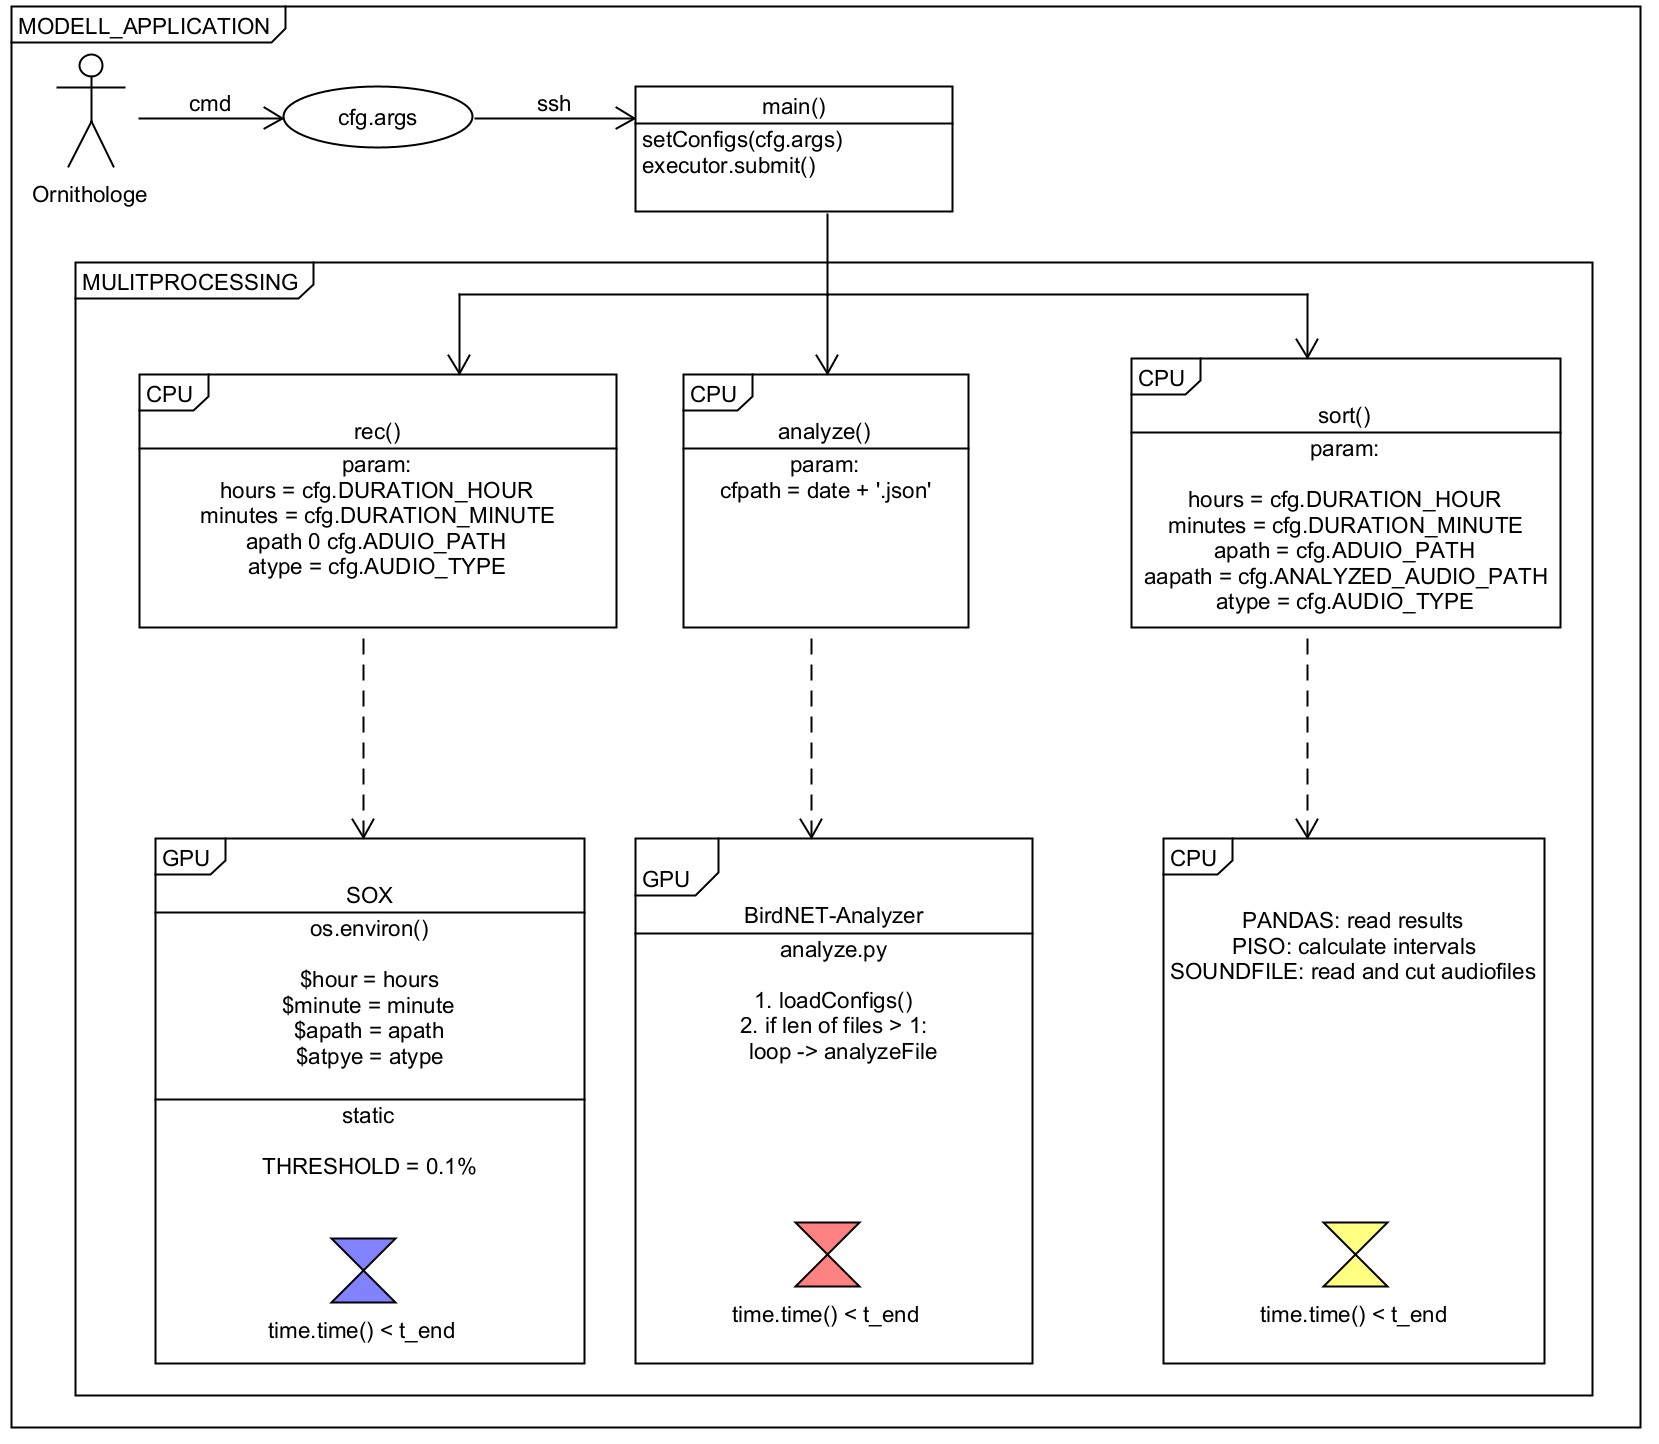
\includegraphics[width=1\linewidth]{bilder/modell_app_2.png}
 \caption{Modell der Applikation}
    \label{fig:versuchsaufbau}
\end{figure}

Das Aktivitätsdiagramm in Abbildung \ref{fig:versuchsaufbau} skizziert den Versuchsaufbau. 

Der*Die Ornithologe*in gibt manuell den Befehl auf dem lokalen Rechner ein. Der lokale Rechner ist mit dem kabellosen Netzwerk des mobilen Computers verbunden und sendet über dieses Netzwerk den Befehl an den Computer. Somit ist dieser der SSH-Server, der für die Datenannahme per SSH-Tunnel und Datenverarbeitug per Software (s. Abschnitt \ref{sec:umsetzung}) zuständig ist. Der mobile Computer ist an eine Powerstation verbunden (s. Abschnitt \ref{subsec:Stromversorgung}). Das Mikrofon ist per USB-Kabel an den Computer angeschlossen (s. Abschnitt \ref{subsec:mikrofon}).


\subsection{Computer \label{subsec:Computer}}
Als mobiler Computer kommt der Nvidia Jetson in der Version Nano J1010 zum Einsatz. 

Damit er sicher in der Box gelagert ist, sitzt er in einem Aluminiumgehäuse. Zudem ist eine Referenz-Trägerplatte von Seeed und ein passiver Aluminium-Kühlkörper eingebaut. Zur Speichererweiterung ist eine SD-Karte im Gerät hinzugefügt.

Um eine kabellose Übertragung der Daten vom Host zum Server zu ermöglichen, ist noch eine WiFi-Karte an den mobilen Computer angeschlossen (s. Abbildung \ref{fig:versuchsaufbau}).

Durch seine technischen Eigenschaften ist der Nano in seiner Performance für KI-Anwendungen geeignet. Es sei jedoch nochmal auf Abschnitt \ref{subsubsec:} hingewiesen.

Der Link zum Datenblatt befindet sich im Anhang \ref{anh:Datenblatt} \cite{jetson_datasheet}.

Alle technisch relevanten Daten sind auch auf der Seite von Nvidia gelistet \cite{jetson_web}.

Das Betriebssystem ist Linux mit Ubuntu 20.04.


\subsubsection{Nutzung eines Hardwarebeschleunigers}
\label{subsubsec:}
Ursprünglich war geplant den Nvidia Jetson Nano aufgrund seiner GPU als Hardwarebeschleuniger und der damit einhergehenden Performanceverbessung für KI-Anwen\-dung\-en zu nutzen. Jedoch hat sich im Laufe der Entwicklung dieses Projektes herausgestellt, dass Nvidia den Support, um Tensorflow %anmerkung was tensorflow ist
auf der GPU laufen zu lassen, nicht (mehr) anbietet. Auch der Umweg durch Installationsanweisungen von anderen Quellen wie von \cite{qengineering}
lohnen sich nicht, da laut diesen Quellen die GPU einen negativen Effekt auf die Rechengeschwindigkeit hat.

\subsection{Stromversorgung \label{subsec:Stromversorgung}}
Für die Stromversorgung im Freien kommt eine Powerbank zum Einsatz. Die wichtigste Anforderung an die Powerbank ist die ausreichende Stromkapazität.
Da der Jetson einen Leistungsverbrauch von 5 bis 10 Watt pro Stunde bei Auslastungen wie KI-Berechnungen oder High Perfomance Computing hat, kommt eine Powerbank mit \SI{266,4}{\watt\hour} zum Einsatz. 
%https://www.nvidia.com/de-de/autonomous-machines/embedded-systems/jetson-nano/product-development/
Durch einen praktischen Versuch ist verifiziert, dass die Stromkapazität der Powerbank ausreicht.

\subsection{Mikrofon}
\label{subsec:mikrofon}

Das Mikrofon hat die Rolle der Datenerfassung inne. Es zeichnet das umliegende Audiosignal auf und leitet es per USB-Kabel an den mobilen Computer weiter. 
Das hier gewählte Mikrofon \textsc{Clippy EM272Z1 Mono} \cite{clippy_microphone} und der dazugewählte Windschutz \cite{soundscapes_windshield} eine Empfehlung vom gekennzeichneten
Amateurfunker \cite{amateurfunker}.
Durch eigene Testversuche ist nach persönlichem Ermessen die Qualität des Mikrofons ausreichend.

%\flqq ausreichend \fqrr\ klassifiziert.


\subsubsection{GPS-Gerät}
\label{subsec:gps}
Zur Erfassung der Koordinaten ist ein GPS-Gerät angeschlossen. Diese Koordinaten verhelfen zu einer sicheren Vorhersage des Neuronalen Netzes. Zudem ermittelt es für den Computer die aktuelle Uhrzeit, da dieser %Verweis auf den Computer?
keine Echtzeit-Uhr verbaut hat. Die Nutzung der Daten vom GPS in der Software sind in Abschnitt \ref{subsec:configs} erklärt.


  % Abschnitt 4: Umsetzung
  \clearpage
  \section{test}

\lstinline{testtesttesttesttesttesttesttesttest}


\section{Umsetzung}
\label{sec:umsetzung}
Dieser Abschnitt beschäftigt sich mit der softwarebasierten Umsetzung. Nach einer allgemeinen Übersicht über den Ablauf des Programms, gehen die Unterabschnitte auf die einzelnen Funktionen und die implementierten Bibliotheken ein.


\subsection{Modell der Software}
\label{subsec:softwaremodell}

\begin{figure}
    \centering
    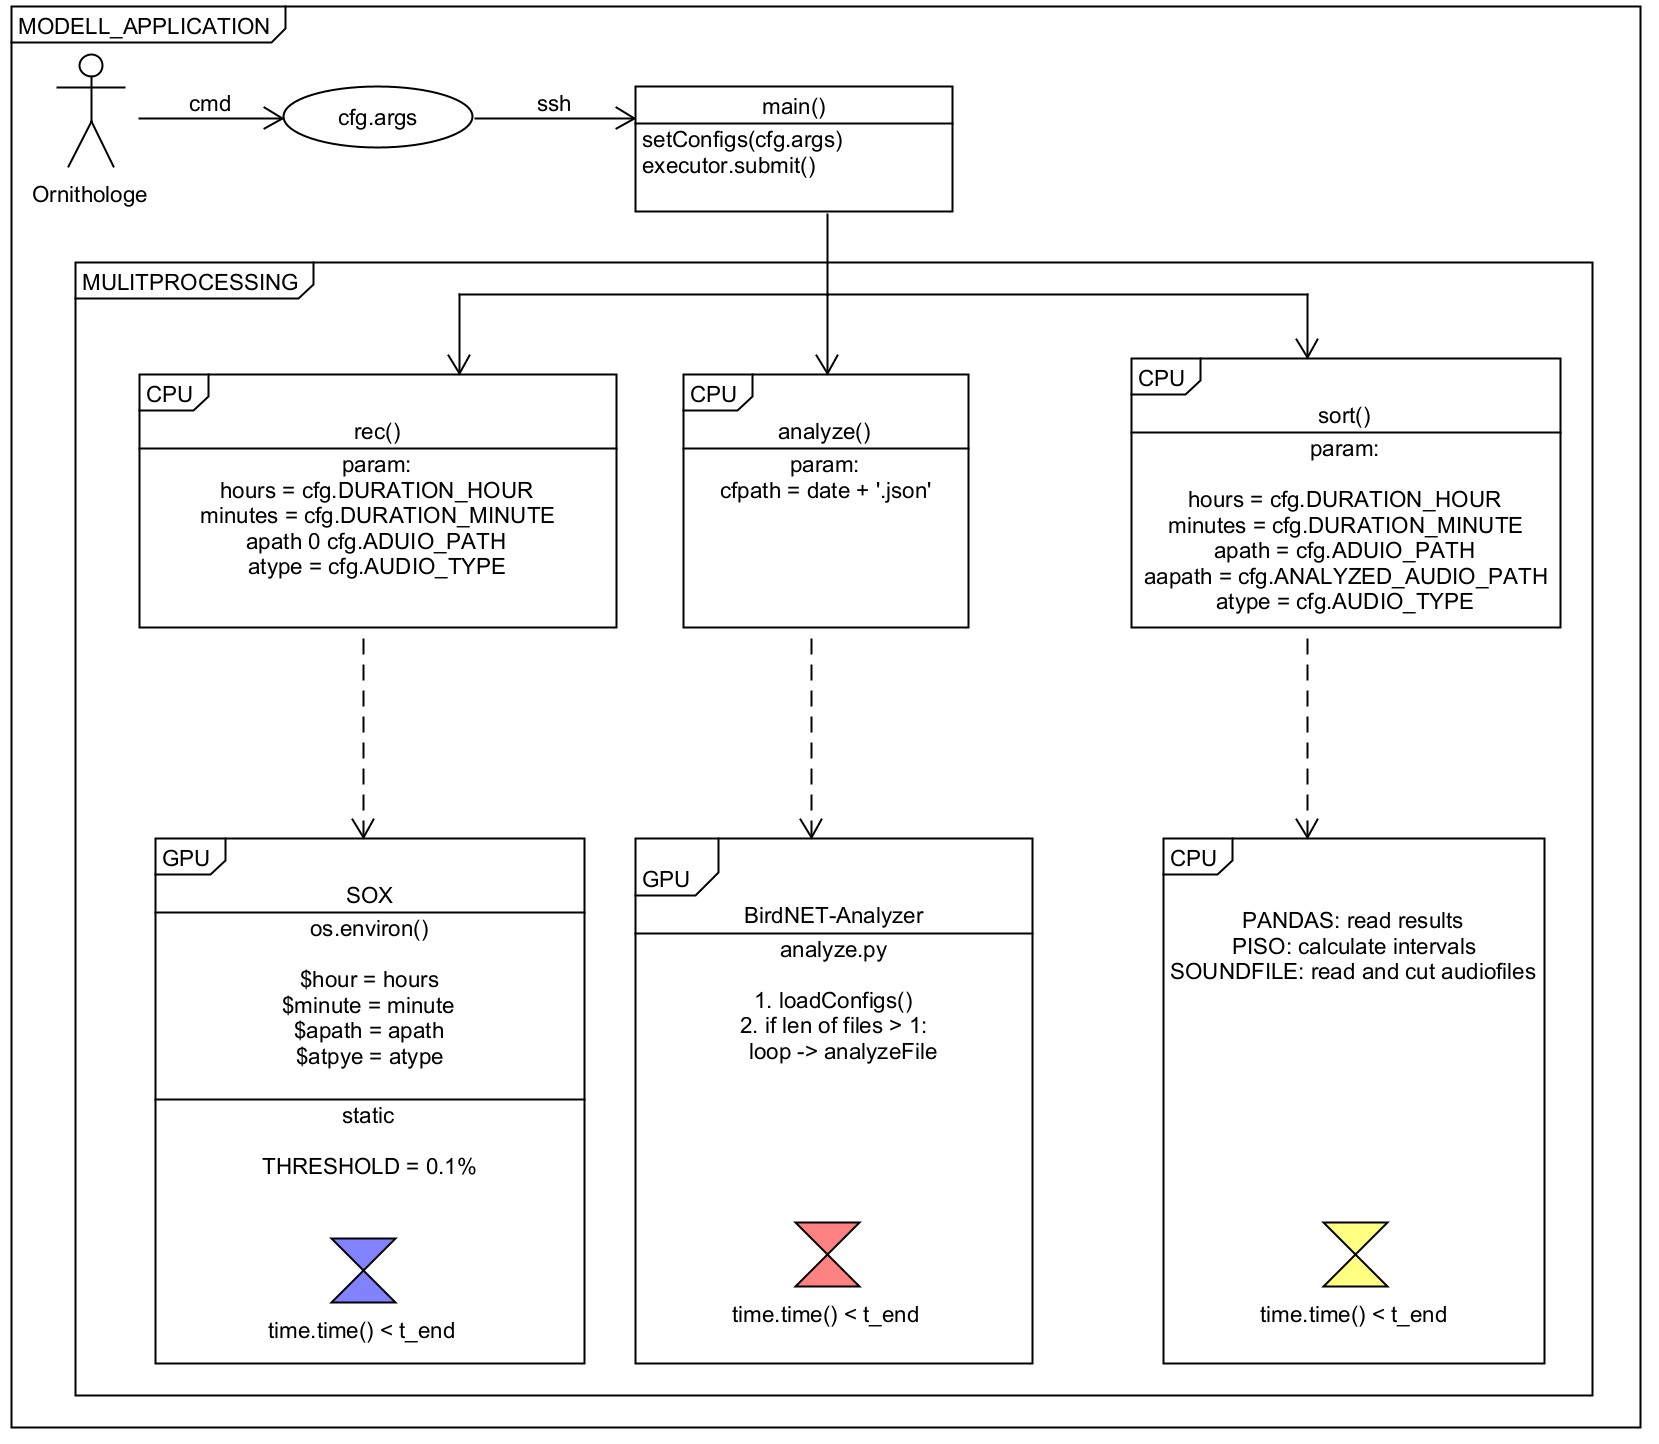
\includegraphics[width=1\linewidth]{bilder/modell_app_2.png}
 \caption{Modell der Applikation}
    \label{fig:model_app}
\end{figure}
%noch so farblich markieren was Initialiserung, Analyse, Aufnahme und Weiterverarbeitung sind
%nochmal alle Titel der Absätze auch im Modell erwähnen

Der*Die Ornithologe*in ruft per Shell das Pythonskript \texttt{main.py} mit den optionalen Startargumenten (s. Abschnitt \ref{subsec:configs}) auf. Beim Aufruf von main.py konfiguriert die main-Funktion das Programm mit den übergebenen Startargumenten. Danach ruft die Funktion über die Methoden der Pythonbibliothek \textit{multiprocessing} (s. Abschnitt \ref{multiprocessing}) die Funktionen \texttt{rec()}, \texttt{analyze()} und \texttt{sort()} als parallel auszuführende Prozesse auf. Diese Funktionen bekommen die Parameter, die im Modell \ref{fig:model_app} in den jeweiligen Blöcken unter \texttt{param:} gelistet sind, übergeben. Die Ausführung der Funktionen ist zeitlich eingegrenzt. Diese wiederum rufen Unterprozesse auf. 


% \begin{python}
% class MyClass(Yourclass):
%     def __init__(self, my, yours):
%         bla = '5 1 2 3 4'
%         print bla
% \end{python}


\texttt{rec()} ruft SOX (s. Abschnitt \ref{subsubsec:sox})  für die energiesparende kontinuierliche Audioaufzeichnung auf. \texttt{analyze()} stellt die Schnittstelle zum BirdNET-Analyzer her (s. Abschnitt\ref{subsec:änderungen}). 

\texttt{sort()} nutzt zum Zuschneiden der Audiofiles die Bibliotheken Pandas (s. Abschnitt \ref{subsubsec:pandas}), Piso (s. Abschnitt \ref{subsubsec:piso}) und Soundfile (s. Abschnitt \ref{subsubsec:soundfile}).


\subsection{Bibliotheken}
\label{sec:bibliotheken}

\subsubsection{Multiprocessing}
\label{subsubsec:multiprocessing}
Multiprocessing ist das zeitlich parallele Ausführen von Prozessen. Python bietet dafür die Bibliothek \texttt{concurrent.futures}. Über das Objekt \texttt{ProcessPoolExecutor} ist die Funktion \texttt{submit()} aufrufbar. Diese Funktion erwartet als Übergabeparameter den Prozess und die Parameter, die an den Prozess zu übergeben sind. Ihre Aufgabe ist die Aufstellung eines Future-Objekts, das die Ausführung des Prozesses darstellt \cite{multiprocessing_doc}.
% https://docs.python.org/3/library/concurrent.futures.html

\subsubsection{Pandas}
\label{subsubsec:pandas}
Pandas ist eine für Python bekannte Bibliothek. Ihre Funktionen sind die Analyse, Verarbeitung und Darstellung von Daten. Insbesondere bietet sie Funktionen und Datenstrukturen für Berechnungen mit numerischen Tabellen und Zeitreihen \cite{pandas-kurs}.
Pandas liest csv-Dateien mit \texttt{read\_csv} \texttt{(filepath\_or\_buffer, sep=\_NoDefault.no\_default)} als DataFrame ein und verarbeitet diesen mit seinen eigenen zahlreichen Funktionen. %hier Quellenangabe: https://pandas.pydata.org/pandas-docs/stable/reference/api/pandas.read_csv.html
Der Übergabeparameter \texttt{sep} erwartet zur Kennzeichnung einen String, mit dem die einzelnen Elemente in der csv-Datei, welche den zugehörigem Dateipfad \texttt{filepath\_or\_buffer} hat, separiert sind.

\lstinline{Series.unique()} gibt eindeutige Werte einer panda-Series zurück als pd.Series\footnote{import pandas as pd}.

Außerdem erstellt die Funktion \lstinline{pd.arrays.IntervalArray.from_arrays()} aus zwei \myPython(arrays) die linke und rechte Grenze eines Intervalls und gibt diese als panda-Daten\-struk\-tur \myPython{IntervalArray} zurück.

Pandas bietet zudem die Funktion \texttt{groupby()} an. Diese ordnet ein DataFrame mit Hilfe eines Mappers oder der Spalte einer panda-Series zu einer Gruppe zu.

Die Funktion \texttt{apply()} wendet eine Funktion entlang einer gewählten Achse eines DataFrames an. Das an die Funktion übergebene Objekt ist demnach eine panda-Series. 

Eine weitere für dieses Projekt hilfreiches Funktion ist \texttt{pd.to\_datetime()}, die eine Datumsangabe zu einem datetime-Objekt von Pandas umwandelt. Diese Datumsangabe kann z.~B. vom Typ \texttt{datetime} sein. Diese Datenstruktur ist von der Biblitiothek \texttt{datetime} (s. Abschnitt \ref{subsubsec:datetime}).


%schreibt man das?
Eine detailreichere Übersicht zu den genannten und weiteren Funktionen von Pandas stellt die Dokumentation von Pandas zur Verfügung \cite{pandas_doc}. %Quellenverweis
%wie die mehreren Quellen angeben?
% idee: diese und weitere Informationen sind unter der Documentation von Pandas zu finden

% https://pandas.pydata.org/pandas-docs/stable/reference/api/pandas.DataFrame.groupby.html


\subsubsection{Soundfile}
\label{subsubsec:soundfile}

Soundfile schreibt mit \lstinline{write()} und liest mit \lstinline{read()} Audiosignale in eine und aus einer Audiodatei. Diese Bibliothek ist für die Soundverarbeitung innerhalb Pythons geeignet, denn sie wandelt Audiosignale in numpy-Arrays\footnote{eine weitere Datenstruktur aus der Bibliothek numpy für Python} um. 

 \texttt{Übergabeparameter:}
 
 \texttt{file: Any} Angabe des Dateipfades
 
\texttt{data: Any}  numpy-Array mit den Daten des Audiosignals

 \texttt{samplerate: Any} Anzahl der Samples pro Periode

\texttt{start: int = 0} Startpunkt, ab dem das Audiosignal einzulesen ist. Angabe in Samples.

\texttt{stop: Any | None = None} Endpunkt, bis zu dem das Audiosignal einzulesen ist. Angabe in Samples. 

Für \texttt{start} und \texttt{stop} gilt: Ein negativer Wert zählt die Samples startend vom Audiosignalende.

\lstinline{Write()} bekommt die Parameter  \texttt{file}, \texttt{data}  und \texttt{samplerate} übergeben und liefert None zurück.
\lstinline{read()} bekommt die Parameter  \texttt{file},  \texttt{start}, \texttt{stop} übergeben und gibt ein Tupel mit den Audiodaten als \texttt{ndarray} vom Typ \texttt{float64} und die Samplerate zurück.

 % Quelle: https://python-soundfile.readthedocs.io/en/0.11.0/#module-soundfile



\subsubsection{datetime}
\label{subsubsec:datetime}

Die Python-Bibliothek \texttt{datetime} ist zum Arbeiten mit Daten und Zeiten. %Sowohl die aktuelle Uhrzeit ist aufrufbar als auch Zeitdifferenzen berechenbar. 
Die Bibliothek stellt einige Objekte wie \texttt{datetime} oder \texttt{timedelta} zur Verfügung, die den Zugriff auf verschiedene Funktionen, Konstruktoren und Attribute ermöglicht. 
\texttt{datetime.} \texttt{timedelta} bekommt Werte für verschiedene Zeiteinheiten (die kleinste Zeiteinheit ist Millisekunden) und berechnet daraus eine Dauer um z.~B. Zeitdifferenzen zwischen zwei \texttt{datetime}- oder \texttt{date}-Objekten zu berechnen.

\begin{python}
    class datetime.timedelta(days=0, seconds=0, microseconds=0, milliseconds=0, minutes=0, hours=0, weeks=0)
\end{python}
            
Zum Erstellen einer \texttt{datetime} oder einer \texttt{date} gibt es das Objekt datetime.datetime, welche Werte für Zeiteinheiten bis Mikrosekunden als kleinste Zeitheintheit bekommt.

\begin{python}
    class datetime.datetime(year, month, day, hour = 0, minute = 0, second= 0, microsecond = 0, tzinfo = None, *, fold = 0)
\end{python}
%A datetime object is a single object containing all the information from a date object and a time object.



Zum Aufrufen der aktuellen Zeit ist datetime.now() verwendbar. Um die aktuelle Zeit in einer spezifischen Format als String zu speichern, ist die Funktion strftime() zu nutzen. Beispielsweise erstellt der Befehl 
\begin{python}
datetime.datetime.now().strftime("%Y%m%d")
\end{python} 
ein Datum mit der Angabe von Jahr, Monat und Tag. Die Angabe von \%Y, \%m und \%d repräsentieren die unterschiedlichen Zeiteinheiten. Die Informationen über die unterschiedlichen Bezeichnungen sind der Tabelle aus deren Dokumentation zu entnehmen \cite{datetime_doc}.

\myPython{strptime()} bewirkt das Gegenteil. Diese Funktion nimmt ein Datum in einer bestimmten Formatierung als ersten Übergabeparameter entgegen. Der zweite Übergabeparameter teilt der Funktion mit, in welchem Format das Datum gespeichert ist, damit die Funktion daraus die Werte der einzelnen Zeiteinheiten interpretieren und auslesen kann \cite{datetime_doc}.

%\myBash[basicstyle=\ttfamily, showstringspaces=false, commentstyle=\color{red}, keywordstyle=\color{blue},  breaklines=true]{datestamp = datetime.datetime.strptime(file_datestamp[0], '%YY%mM%dD%Hh%Mm%Ss%fms')}


\subsubsection{ALSA}
\label{subsubsec:alsa}
ALSA ist eine unter Linux integrierte Soundsystemarchitektur. Sie besteht aus Linux-Kernelmodulen und betreibt Soundkarten. 
% nomankaltur? \textbf{A}dvanced \textbf{L}inux \textbf{S}ound \textbf{A}rchitecture
Mit den Funktionen von ALSA ist es möglich, Audio aufzunehmen und abzuspielen \cite{alsa_doc}. Mehr dazu in Abschnit /ref{subsubsection:sox}.

\subsubsection{glob}
\label{subsubsec:glob}

Die Python-Bibltiothek glob bietet die Funktion glob(pathname, [...]).

Damit sind alle Pfadnamen, die einem vorgegebenen Muster entsprechen, auffindbar. Das Muster gestaltet sich nach den Vorgaben der Unix-Shell für Pfadangaben. Die Reihenfolge der gefundenen Pfade ist zufällig.

Platzhalter für variable (Pfad-)Angaben sind \textbf{*}, \textbf{?}, \textbf{[]}. Letzteres ist Platzhalter für Zeichenbereiche \cite{glob_doc}.

    
\subsubsection{Sox}
\label{subsubsec:sox}
Sox ist ein Audiotool zur Verarbeitung von Audios mit Filtern und Soundeffekten während der Konvertierung.

%Sox kommt in diesem Projekt als Aufnahmesoftware und Audiovorverarbeitung zum Einsatz. 
Mithilfe des Effekts \textit{silence} verwirft Sox Audioabschnitte, in denen Stille herrscht, schon während der Konvertierung. 
Die Synopsis, der Befehle für die Audioaufzeichnung, ist wie folgt aufgebaut:

%\begin{bash}[caption={Synopsis der Befehle für das Aufzeichnen von Audio mit Sox}]
    
    sox [global-options] [format-options] infile1 [[format-options] infile2] ... [format-options] outfile [effect [effect-options]] ...

rec [global-options] [format-options] outfile [effect [effect-options]] ...

%\end{bash}


Beide Befehlen zeichnen Audio auf. 

Die für dieses Projekt relevanten Operationen sind:

\textbf{-t} Festlegung, mit welchem Audiogerät und Audioaufnahmesoftware Sox aufnimmt

\textbf{-r} Angabe der Samplerate, welche für die Anzahl an Samples pro Periode steht

\textbf{-b} Anzahl der Bits, mit denen ein Sample codiert ist

\textbf{-e} Audiodekodierungstyp. 
 Mit der Angabe von \textbf{signed-integer} ist festgelegt, dass die PCM\footnote{Pulse Code Modulation} %nomenklatur?
 -Daten als vorzeichenbehaftete Ganzzahlen zu speichern sind. In der Regel kombiniert man diese Angabe mit einer 16- oder 24-Bit-Codierungsgröße. Hierbei steht der Wert null für die minimale Signalleistung.


\textbf{silence} Effekt zum Trimmen von Stille während der Aufnahme. 
Die Synopse lautet:

\begin{lstlisting}[language=bash,caption={Synopse für den Befehl von Stille während der Konvertierung},]
[-l] above-periods [duration threshold[d|%] [below-periods duration threshold[d|%]]
\end{lstlisting}
Die relevanten Operationen von \textbf{silence} sind: % oder texttt

\textbf{above-periods} Audio ist am Anfang der Audio zu trimmen. Der eingestellte Wert legt fest, wie oft am Anfang Stille zu trimmen ist. Bei einem Wert von null ist das Trimmen ausgeschaltet, bei eins passiert es nur einmal. Ist der Wert größer als eins, schneidet sox mehrere Stellen mit Stille ab Audioanfang raus.

\textbf{duration} Zeitangabe, wie lange Stille in einem Audiosegment kontinuierlich herrschen muss, damit Sox dieses entfernt.

\textbf{threshold} Schwellwert für die Lautstärke. Ton unter diesem Wert ist als Stille definiert.

\textbf{below-periods} Aufnahme ist am Ende der Audio zu trimmen. Der eingestellte Wert legt fest, wie oft am Ende Stille zu trimmen ist. Die Einstellung des Wertes funktioniert genauso wie bei \textbf{above-periods} nur rückwärts beginnend bei Audioende.

\textbf{: newfile : restart} Dieser Befehl bewirkt einen Ketteneffekt durch den Operator \textbf{:} .  Mit \textbf{newfile} erstellt Sox aus der durch den vorherigen Effekt verarbeiteten Audio eine neue Audiodatei. Jede neu erstellte Audiodatei bekommt am Dateinamensende eine eindeutige Nummer angehängt. Danach springt Sox mit \textbf{restart} zum ersten Effektkettenglied. Der Prozess wiederholt sich.

Beispielsweise kann ein Befehl für das Trimmen von Audio während der Aufzeichnung wie folgt geschrieben sein:
\begin{lstlisting}[language=bash,caption={Besipiel eines SOX-Aufrufs mit Trimmen von Stille während der Konvertierung},]
sox -t alsa hw:2,0 -r 48000 -b 16 -e signed-integer "song.wav" silence 1 0.50t 0.1% 1 2.0 0.1% : newfile : restart
\end{lstlisting}

%lieber in der Erklärung der Software
Dieser Befehlszeile nimmt als default-Gerät ein extern eingestecktes Mikrofon mit der Kartennummer 2 und der Gerätenummer 0, gekennzeichnet durch \lstinline{hw:2,0}, und als Soundsystem \textbf{alsa}. 
%Überhaupt erwähnen?
Die von \textbf{alsa} erkannten Geräte mit den jeweiligen Nummerierungen von Karte und Gerät sind unter dem Befehl \lstinline{arecord -l} zu finden. 

\lstinline[caption=Beispiel für eine mögliche Ausgabe]{card 2: Device [USB PnP Sound Device], device 0: USB Audio [USB Audio]}


\subsubsection{gps}
\label{subsubsec:gps}
Für Python gibt es die Bibilothek gps

- Einlesen der Daten, die das GPS Gerät ermittelt und an den Computer sendet
- Mit den Funktionen latitude, Longitude und Uhrzeit auslesen
- funktion zum Prüfen, ob das Gerät erkannt wurde oder so % also alle gneutzen Funktionen erklären

Die Einbindung der Bibliothek und Datenauslesung des GPS-Geräts findet in Abschnitt ... statt.


\subsubsection{Piso}
\label{subsubsec:piso}

Piso unterstützt die Berechnung von Intervallklassen in Pandas für Mengenoperationen wie Vereinigungs- oder Schnittmenge.

Die Funktion \lstinline{piso.register_accessors()} ermöglicht Piso den Zugriff auf \lstinline{pd.arrays.IntervalArray}. 

union
Die Zusammenführung der Intervalle passiert durch die Funktion union, die bekommt ... übergeben und verbindet Intervalle mit gemeinsamen Schnittstellen.


\subsection{Initialisierung}
\label{sec:Initialisierung}

% wohin mit dem Abschnitt Start per kabelloses Netzwerk?

Das Modell \ref{fig:model_app} zeigt, dass die Initialisierung von main.py in drei zusammenfassende Schritte unterteilt ist:

\begin{enumerate}
    \item Start des Programms über einen Shell-Befehl
    \item Einlesen der Startargumente und konfigurieren
    \item Start der drei parallelen Prozesse mit dem \myPython{ProcessPoolExecutor()} aus der //concurrent.futures-Bibliothek
\end{enumerate}


Der Start des Programms über die Shell ist am Ende diese Kapitels in Abschnitt \ref{subsubsec:start} erklärt.

Schritt 2 passiert drei Unterschritte.

Mit
\begin{lstlisting}
    parser = argparse.ArgumentParser(description="Start audio recording session")
\end{lstlisting}

kann \lstinline{main.py} auf die Startargumente zugreifen.
Danach ist festgelegt, wie mit diesen Startargumenten umzugehen ist. Ein Startargument ist \texttt{region}.
%beispiel dazu noch
\begin{python}
parser.add_argument(
        "--region", default="COUNTRIES/world/", help="Path to folder where audiofiles, analyzed audiofiles and results are saved."
)

cfg.REGION = args.region{}

\end{python}

Hier ist festgelegt, dass der Default-Wert von \texttt{region} ein Dateipfad ist. Dieser Wert wird als Konfiguration in \lstinline{config.py} gespeichert.

%hier das GPS Gerät erwähnen

% Schritt 2
Wenn das Startargument \texttt{-{}-config} mit dem Wert True übergeben ist, versucht das Programm die Koordinaten und die Zeit vom GPS-Gerät für die Postfilterung zu Nutzen. Was die Postfilterung ist, erklärt Abschnitt \ref{subsubsec:speiceslist}. Da das Gerät aber nicht sofort und überall Koordinaten findet, wartet die Funktion \myPython{getCoordinates()} nach diesen solange, bis der*die Anwender*in diesen Vorgang abbricht oder das GPS-Gerät die Koordinaten gefunden hat. Bricht der*die Anwedner*in das Programm vorher ab, fragt jenes ihn*sie, ob es die Audiosession dennoch fortgeführt werden soll oder abbrechen soll. Hierfür ist der*die Anwender*in zur Eingabe aufgefordert. \textit{y} steht für \textit{yes} und \textit{n} für \textit{no}.
Hat der*die Anwender*in die Startargumente \texttt{-{}-lat}, \texttt{-{}-lon} und \texttt{-{}-week} übergeben, nutzt das Programm diese, ansonsten nutzt es die Default-Werte, die alle minus eins sind und somit nutzt das Modell keine Koordinaten für die Vorhersage. Sollte das GPS-Gerät die Zeit nicht finden, wird die Offline-Zeit genutzt. Bei Diskrepanz mit der Echtzeituhr ergibt sich ein Zeitfehler, der bei der Auswertung nach der Audiosession zu beachten ist.

\myPython{def getCoordinates()}


%schritt 3
Zum Speichern der Config-Datei ist in main.py die Funktion \myPython{saveConfigsAsJSON(configs:str, cfpath:str)} definiert. Diese erwartet für den Parameter \myPython{configs} das Dictionary mit den Konfigurationen, aufrufbar über die Funktion \myPython{getConfigs()} von \myPython{config.py}, und den Dateinamen der JSON-Datei, in den sie das Dictionary schreiben soll.

\begin{python}
    def saveConfigsAsJSON(configs: Dict, cfile_path: str):
        configs_json = json.dumps(configs)
        with open(cfile_path, 'w') as cfp: 
            cfp.write(configs_json)
            
    configs = cfg.getConfig()
    cfname = datetime.now().strftime("%Y%m%d") + '.json' # configs_filename
    cfpath = os.path.join('configs_files', cfname)
    saveConfigsAsJSON(configs, cfpath)

\end{python}

Schritt drei ist der Aufruf aller drei Parallelprozesse.

%Dabei ist bewusst zuerst analyze aufgerufen, um zu ermöglichen, dass erst das Netz geladen wird, bevor die Audiosession mit der Aufnahme anfängt. Dies ist für die nicht so relevanten Prozesse ein Zeitvorteil
%noch umsetzten und testen!

\begin{python}
      with concurrent.futures.ProcessPoolExecutor() as executor:
        p2 = executor.submit(analyze, cfpath)
        p1 = executor.submit(rec, cfg.DURATION_HOURS, cfg.DURATION_MINUTES, cfg.AUDIO_PATH, cfg.AUDIO_TYPE)
        p3 = executor.submit(slice_audio, hours = cfg.DURATION_HOURS, minutes = cfg.DURATION_MINUTES, apath = cfg.AUDIO_PATH, aapath = cfg.ANALYZED_bei seinemAUDIO_PATH, atype = cfg.AUDIO_TYPE)
\end{python}


\subsection{Aufnahme}

\subsubsection{Programmfunktionen und -parameter sowie Sox-Aufruf}
Für die Aufnahme ruft \textit{main.py} die Funktion \myPython{rec()} auf. 

%\begin{python}{def rec(hours: int, minutes: int, apath: str, atype:str)} \end{python}

Die Werte der übergebenen Parameter \texttt{audio\_path} und \texttt{atype} initialisieren die Umgebungsvariablen  \texttt{audio\_path} und \texttt{audio\_type}. Diese nutzt Sox (s. Abschnitt \ref{subsubsec:sox}) bei seinem Aufruf. 


\begin{bash}[frame=shadowbox]
    sox -t alsa hw:2,0 -r 48000 "$audio_path$(date +"%YY%mM%dD%Hh%Mm%Ss%3Nms_").$audio_type" silence 1 0.50t 0.1% 1 2.0 0.1% : newfile : restart
\end{bash}


Der Datumsstempel ist im Dateinamen festgehalten, um später wie in Abschnitt \ref{subsec:änderungen} erwähnt, einen Datumsstempel in der Ergebnistabelle hinzuzufügen.

Umgeben ist der Aufruf der Funktion mit dem Zeitbegrenzer.

\begin{python}
    t_end = time.time() + hours * 3600 + minutes * 60
    while time.time() < t_end: 
        # rufe sox auf    
\end{python}


\subsubsection{Mikrofonrauschen und Schwellwertanpassung}
\label{subsubsec:mikrofonrauschen}
Der gewählte \texttt{threshold} soll den Schwellwert für Stille festlegen. Da analoge Audio immer mit einem Rauschen durch das Mikrofon unterlegt ist, ist der Schwellwert mit einer bestimmten Toleranz zu wählen. Diese kann der*die Anwender*in selbst einstellen, da jedes Mikrofon durch seine Eigenschaften unterschiedlich starkes Rauschen verursacht. Für das hier gewählte Mikrofon ist durch Testversuche der \texttt{threshold} von \texttt{0,062} gewählt, das der Rauschlautstärke des Mikrofons näherungsweise entspricht. Schwellwert soll also die Lautstärke des Rauschens selbst sein.
Zur Bestimmung dieses Wertes ist das Rauschen aufzunehmen und daraus ein Mittelwert zu ermitteln. Es bedarf aber noch einige Versuche diesen Wert anzupassen bis das Ergebnis zufriedenstellend ist. Da auch das Rauschen kein konstanter Wert ist, sollte eine ausreichende Toleranz über die durchschnittliche Rauschlautstärke gewählt sein.

\subsection{Analyse}


\subsubsection{Vorstellung des BirdNet-Analyzers}
\label{subsubsec:vorstellung}

Für die Erkennung von Vogelgesang nutzt die Software das Modell vom BirdNET-Analyzer \cite{kahl2021birdnet} sowie weitere Programme und Funktionen von dessen API. Die erste Gitversion heißt BirdNET, ist aber veraltet. Die neue Version ist unter dem Namen BirdNET-Analyzer herausgegeben. Die Entwickler geben an, diese Version weiterhin zu updaten.

Wie BirdNET grob funktioniert, beschreiben die folgenden Zeilen. Für genauere Information über BirdNET, wie es zu installieren und anzuwenden ist, ist auf das Git-Repository \cite{birdnetGit} verwiesen.


%wie funktioniert BirdNET -> erklären, wie es angewandt
%Zum Analysieren von Audiofiles ist das Programm analyze.py mit den entsprechenden Startargumenten aufzurufen. Die verschiedenen Startargumente sind für verschiedene Einstellungen. 
%Als Beispiel :

%python3 analyze.py --i example/ --o example/

%muss man das erklären?
%noch hinzufügen was --i und --o sind
%Dieser Terminalbefehl ruft analyze.py auf und compiliert ihn mit Python3. Dabei liest analyze.py die Startargumente ein. Als Input ist der Ordner example angegeben (gekennzeichnte mit \texttt{--i} davor), aus dem das Programm alle vorhandenen Audiofiles analysiert. Dabei müssen die Audiosignale in 48000 Hz  kodiert sein. Bei der Analyse schneidet das Programm die Audio in Drei-Sekunden-Segmente und speist sie dann ins neuronale Netz. Die Ergebnistabelle der analysierten Audio ist im Ornder \texttt{example} gespeichert (gekennzeichnet mit \texttt{--i} davor). 

%kürzere Version
Über verschiedene Terminalbefehle sind verschiedene Programme und Funktionen vom BirdNET-Analyzer aufrufbar. Zur Analyse von Audiodateien ist das Pythonskript \textit{analyze.py} mit den gewünschten Einstellungen übergeben als Startargumente aufzurufen.


Informationen zu allen Startargumenten ist in der ReadMe im Git von BirdNET zu finden.

Nach der Analyse der Audiodatei(n) gibt BirdNET die Default- oder vom Anwendenden gewünschte Ergebnistabelle zurück. 
Je nach Ergebnistabelle können bei jeder erkannten Vogelart in einem bestimmten Zeitabschnitt in der Audio verschiedene andere Informationen hinterlegt sein, die zur Weiterverarbeitung nutzbar sind. 



\subsubsection{Änderungen in BirdNET}
\label{subsec:änderungen}

Das Schaubild %besseres Wort?
\ref{fig:model_app} zeigt, dass die Funktion \myPython{analyze()} aus \myPython{main.py} die Schnittstelle zum BirdNET-Analyzer ist. 

Bei Aufruf von \myPython{analyze()}, ruft diese wiederum per Shell-Befehl das Programm \textit{analyze.py} von BirdNET auf.
%erwähnen dass es mit os.system gemacht wird?
Statt wie vorher in Abschnitt \ref{subsubsec:vorstellung} gezeigt, die Startargumente an \textit{analyze.py} zu übergeben, bekommt \textit{main.py} diese Startargumente und lädt sie als JSON-Datei in den Ordner \textit{configs-files}.
Diese Änderungen hat den Vorteil, dass die Einstellungen wiederverwendbar sind. Auf die genaueren Umsetzung geht der Abschnitt \ref{subsec:configs} ein.



\myPython{analyze()} bekommt den Dateinamen der JSON-Datei übergeben. Mittels des Befehls \myPython{os.system()} ruft sie \textit{analyze.py} auf und übergibt als Startargument diesen Dateinamen. 

\begin{python}

if __name__ == "__main__":
    # Freeze support for executable
    freeze_support()
    
    parser = argparse.ArgumentParser(description="Analyze audio files with BirdNET")
    
    parser.add_argument(
        "--configs",
        type =str,
        default=None,
        help="Path to configs. Defaults to None. If set, --configs is ignored.",
    )

    args = parser.parse_args()
    cfile_path: str = ""
    print(type(cfile_path))
    configs_json = ""
    if args.configs is not None :
        cfile_path = str(args.configs)
        with open(cfile_path, 'r', encoding='utf-8') as cfp:
            configs_json = json.load(cfp)

        cfg.setConfig(configs_json)
    \end{python}

\textit{analyze.py} kann mit der Angabe des Dateinamens auf die gewünschte Konfigurationsdatei zurückgreifen. 



Da es sich bei diesem Vorgehen um eine mehrstündige Aufnahme handelt, sind für eine besseren Auswertung der Ergebnisse % (aus Sicht eines Ornithologen) besser erklären, warum das besser ist
zu den Ergebnistabellen csv, table und R zwei Datumsstempel im UTC-Format beigefügt. 

%Bilder zu den jeweiigen Tabellen

%diesen Absatz erst bei der Versuchsdurchführung
%oder ein extra Kapitel wo erstmal Tests durchgeführt wurden, bevor man mit der tatsächlichen Versuchsdurchführung gestartet hat.
% plus ein Kapitel über die GPU und warum sie nicht nutzbar ist (hersteller bietet dafür den Support nicht mehr an und laut anderen Quellen lohnt es sich nicht, Quellen noch angeben)


%bessere Überschrift
\subsubsection{analyze.py}
Beim den Aufruf von analyze.py sind % # TODO:Text hinschreiben

\subsubsection{Effizienzsteigerung} % TODO: Löschen?
Eine Anforderung des Projekts ist, dass der mobile Computer mit der Stromversorgung der Powerbank für mindestens 24 Stunden auskommt. Zudem soll die Analyse möglichst in Echtzeit und zeiteffizient sein. Um diese Anforderungen zu optimieren, gibt es Tests zu unterschiedlichen Einstellungen und Szenarien, die diese Eigenschaften beeinflussen können. Dazu gehört zum einen die Batchsize. Diese hat eine Effekt auf die Performance des Modells sowie auf die Trainingszeit. Der größte Vorteil einer hohen Batchsize ist, dass Hardwarebeschleuniger wie GPU damit bessere Performance erbringen können sowie einen positiven Effekt auf die Zeit haben.


%zusätzlich mit Einstellen Priorität
%overlap

\section{Erste Versuchsdurchführungen} %FIXME: entweder was zu overlap schreiben oder alles rauswerfen

%hier erklären, dass man versucht hat, die Batchsize, Overlap und GPU zu testen
%die Ergenbnisse validiert und anhand dessen das weitere Vorgehen durchgegangen


Zwar ist der Jetson mit seiner CPU relativ 


Zwar hat der Jetson Nano mit seiner GPU eine hoher Leistungsfähigkeit, dennoch sollen die hier vorgenommenen Test die Effizienz steigern. Dafür ist zum einen die optimale Batchsize bestimmt worden, die mmmm vereint.

default-Wert von Batchsize

sensitivity und overlap haben Auswirkungen auf die Rechenleistung

-> Test und deren Ergebnisse

Auch \texttt{overlap} hat einen Einfluss auf die Zeitperformance des Modells. 
Da das Programm eine Audio immer in Drei-Sekunden-Segmente schneidet, analysiert das Netz auch immer nur diese drei Sekunden. Das hat zum Nachteil, dass eventuell das Programm mitten im Vogelgesang die Aufnahme trennt. Das kann wiederrum negative Effekte auf die Vorhersagbarkeit haben.
%was ist overlap
Mit Overlap ist beeinflussbar, wie das Programm die Audio zuschneidet. Zwar kann das Netz immer nur 3 Sekunden auf einmal analysieren, aber diese 3-Sekunden-Intervall verschiebt sich auf der Audio immer nur um den gegebenen Overlap-Wert. 
Als Beispiel, ein \texttt{overlap} von 0 bewirkt, dass das Programm alle drei Sekunden einen Schnitt macht. Mit einem \texttt{overlap} von 1 startet das Modell die Analyse auch bei zwei Sekunden und analysiert dann in drei Sekundenschritten die Audio.

%noch ein paar Tests mit dem Overlap machen und dann bei der Versuchsdurchführung, also echter Versuch gucken, ob der Jetson damit noch mithält

\subsection{Startargumente und Konfigurationen}
\label{subsec:configs}

Wie schon in Abschnitt \ref{subsec:änderungen} erwähnt, bekommt nicht mehr analyze.py von BirdNET die Startargumente, sondern das Hauptprogramm main.py. 
Diese Startargumente sind in der Konfigurationsdatei \texttt{config.py} von BirdNET hinterlegt.

%erklären, dass diese Startargumente in der Config-Datei hinterlegt sind


Neben dieser Änderung gibt es weitere Änderungen bei den Startargumenten selbst. Das Programm nimmt einige zusätzliche Startargumente an, andere sind aus der Liste entfernt worden.
Diese Änderungen sind in diesem Abschnitt erläutert. 

%Für den Rest auf die ReadMe datei hinweisen -> was soll in der ReadME datei angegeben sein?


Die hinzugefügten Startargumente sind \texttt{-{}-hour}, \texttt{-{}-minute}, \texttt{-{}-region}, \texttt{-{}-atype}, \\\texttt{-{}-coordinates}, \texttt{-{}-trim}, \texttt{-{}-threshold}, \texttt{-{}-rtpye2}, \texttt{-{}-delete}

\texttt{-{}-hour} gibt die Stunden an, die aufzuzeichnen sind. Default-Wert ist null.

\texttt{-{}-minute} gibt die Minuten an, die aufzuzeichnen sind. Default-Wert ist 20.

\texttt{-{}-atype} legt das gewünschte Audioformat fest. Dazu sei angemerkt, dass für jedes Audioformat ein sogenannter \textit{handler} zu installieren ist \cite{debian-libsox}. 

%mehr dazu im ReadME
% Alle handler lassen sich mit dem Befehl sudo apt install libsox-fmt-all installieren
%https://packages.debian.org/sid/libsox-fmt-all
\texttt{-{}-region} gibt an, in welchem Ordner Audioaufnahmen, Ergebnisse und die daraus zugeschnittenen Audios zu speichern sind. Dieser Ornder hat dabei immer zwei Unterordner. In den Unterornder \\\texttt{audiofiles} speichert \myPython{rec()} die aufgenommenen Audios und  nach der Analyse verschiebt \myPython{analyze()} die Audios in den Unterordner \texttt{analyzed\_audiofiles}, wobei jede Audiodatei nochmal in einen eigenen Ordner zusammen mit den dazugehörigen Ergebnissen und den zugeschnittenen Audios gespeichert ist.  Der Default-Wert von \texttt{-{}-region} ist \texttt{COUNTRIES/world}. Dieser Pfad befindet sich auch schon im Projektverzeichnis.

Der Variablenname \texttt{region} soll den*die Anwender*in dazu motivieren, den Ordner nach dem Standortrt zu benennen, wo er*sie die Aufnahme durchgeführt hat. Optimalerweise sollte der Ordner dem Ordner \texttt{COUNTIRES} untergeordnet sein. Damit entwickelt sich eine strukturierte Übersicht über alle Audiosessions, die an verschiedenen Standorten entstanden sind.

\texttt{-{}-coordinates} ist eine boolesche Variable, die bei dem Wert True dem Programm mitteilt, dass es für die Analyse die Koordinaten vom GPS-Gerät nutzen soll. %ein artikel über gps schreiben

\texttt{-{}-threshold} hat einen Default-Wert von 0.062. Dieser definiert den Schwellenwert für den Silence-Effekt wie in Abschnitt \ref{subsubsec:sox} erklärt. Da dieser Wert aber auf das hier genutzte Mikrofon abgestimmt ist, steht dem*der Anwender*in offen, diesen Wert für sein*ihr Mikrofon oder die eigenen Präferenzen anzupassen. So ist es auch möglich mit einem größeren Schwellenwert den Aufnahmeradius einzuschränken und mit einem kleineren Radius zu erweitern.  

\texttt{-{}-trim} legt fest, was die maximale Audiolänge einer einzelnen Aufnahme sein darf, wenn der Silence-Effekt nicht vorhehr selbst die Audio zuschneidet. Damit ist bei einem zu kleinen Threshold für Silence verhinderbar, dass eine Audiodatei zu lang wird oder gar so lang wie die gesamte Audiosession ist.

\texttt{-{}-delete} ist Default auf False, was heißt, dass das Programm die Originalaufnahmen nach der Auswertung nicht löscht. Durch setzen auf True ist das Gegenteil der Fall. Dieses Startargument erfüllt die Anforderungen für die Einhaltung des Gesetztes welches die Vertraulichkeit des Wortes bewahrt.


Entfernte Startargumente sind \texttt{-{}-i} und \texttt{-{}-o}. 
\texttt{-{}-i} gab an, in welchem Ordner sich die zu analysierende Audiodatei befindet.
\texttt{-{}-o} gab an, in welchen Ordner die Ergebnisse der analysierten Audio zu speichern sind.

Zu den hinzugefügten Konfigurationen gehören \lstinline{AUDIO_PATH} und \lstinline{ANALYZED_AUDIO_PATH}. \lstinline{AUDIO_PATH} speichert die Pfadangaben \textit{audiofiles/} und \lstinline{ANALYZED_AUDIO_PATH} \textit{analyzed\_audiofiles/}. Beide Variablen beinhalten also den Pfadnamen des Unterordners von \texttt{-{}-region}.


%\paragraph{Ergebnisse}
% \texttt{-{}-rtype} bestimmt den Typ der Ergebnistabelle. Da das Programm standardmäßig eine CSV für die Ergebnistabelle erstellt, erzeugt dieses bei der Angabe von \texttt{-{}-rtype} zusätzlich eine weitere Ergebnistabelle. Diese sind auswählbar zwischen R, Tabelle, Kaleidoscope und Audacity mittels der jeweiligen Werte [\texttt{r}, \texttt{table}, \texttt{audacity}, \texttt{kaliedoscope}].

\texttt{--rtype} bestimmt den Typ der primären Ergebnistabelle. Zu jedem analysierten Audiosegment erstellt das Programm eine Tabelle, die standardmäßig als CSV formatiert ist. Optional speichert das Programm die Tabelle stattdessen als Plain-Text-Tabelle.

%eventuell prüfen, ob es einen zeitlichen unterschied zwischen table und cvs als Ausgabe gibt. Braucht table länger als csv? Wir wirkt sich die Geschwindigkeit dabei aus, wenn man zwei Tables ausgibt

% \texttt{-{}-rtype2} ist optional. Da zur Auswertung das Programm automatisch entweder eine Tabelle als CSV- oder als Text-Datei erstellt, gibt es das Startargument \texttt{-{}-rtype2}. Jenes legt den Dateityp fest, indem die Ergebnisse zu speichern sind. Je nach Dateityp können die Progamme R, Audacity oder Kaleidoscope diese Ergebnisse lesen und auswerten.

% \texttt{--rtype2} ist ein optionales Startargument. Um eine weitere Tabelle als nur eine CSV oder Table für andere Arten der Auswertung zu erzeugen. Mit Angabe von \texttt{r}, \texttt{kaleidoscope} oder \texttt{audacity} speichert das Programm die formatierte Tabelle in den Formaten \textit{.r}, \textit{.csv} oder \textit{.txt}, welche entsprechend von den Programmen R, Kaleidoscope oder Audacity lesbar sind.

\texttt{--rtype2} ist ein optionales Startargument, das es ermöglicht, zusätzlich zur CSV- oder Plain-Text-Tabelle eine weitere Tabelle für unterschiedliche Auswertungsarten zu erzeugen. Bei Angabe von \texttt{r}, \texttt{kaleidoscope} oder \texttt{audacity} speichert das Programm die formatierte Tabelle in den Formaten \textit{.r}, \textit{.csv} oder \textit{.txt}, die entsprechend von den Programmen R, Kaleidoscope oder Audacity gelesen werden können.

%\paragraph{Wiederverwendung von configs}
\texttt{-{}-configs} ermöglicht die Wiederverwendung von alten Konfigurationen.
Das Programm speichert bei jedem Start die dazu festgelegten Konfigurationen im Ordner \texttt{configs\_files}. Der Dateiname ist das aktuelle Datum. Mit der Angabe des Dateinamens der Konfigurationsdatei, welche dem Muster \texttt{YYYYMMDD.json}\footnote{Y=Jahr (Year), M=Monat (Month), D=Tag (Day)} entspricht, sind alle Konfigurationen von der gewählten Konfigurationsdatei für den neuen Start festgelegt. Trotz Angabe von weitere Startargumenten, ignoriert das Programm jene.
% config\_\%Y\%M\%D.json lieber so?


\subsubsection{Species List}
\label{subsubsec:speiceslist}

Ein Ziel dieses Projektes ist die Differenzierung zwischen Vogel und Nicht-Vogel. Dabei sind alle Audioabschnitte, in denen das Netz ein Vogel erkannt hat, gesondert abzuspeichern und alle Nicht-Vogel zu ignorieren oder sogar zu verwerfen.


Die Liste aller Vogelarten basiert auf der eBird checklist frequency \cite{bird-glossary}. % FIXME: Quelle wird nicht im Verzeichnis angezeigt
Dies ist ein Vogelglossar mit zahlreichen Vogelarten. Zu jeder Vogelart ist mit Angabe von Latitude, Longitude und Kalenderwoche die Wahrscheinlichkeit dessen Auftretens in bestimmten Breiten- und Längengraden zu einer bestimmten Zeit im Jahr hinterlegt. 
Das neuronale Netz ist mit diesen Daten trainiert. Da das Netz aber auch erkennen sollte, wann es sich bei bestimmten Geräuschen um Nicht-Vogelarten handelt, sind in der Liste mit den Klassenvorhersagen auch Nicht-Vogel wie Elektrowerkzeuge  (Power tools) oder menschliche Stimmen (Human vocal). 
%warum soll das Netz nicht-Vogel erkennen
Dies dient beim Training des Netzes dazu, verstärkt den Unterschied zwischen Vogelstimmen und Nicht-Vogelstimmen zu erkennen.

Da also in der Ergebnistabelle auch Nicht-Vogelarten stehen können, die das Programm nach der Analyse zum Zuschneiden der Audios nutzt, sollte das Programm die Nicht-Vogelarten herausfiltern.

Umgesetzt ist das mit einem Postfilter. BirdNET hat ein Startargument \texttt{-{}-slist}. Dieses Argument erwartet einen Pfad zu einer Textdatei, die zur Filterung der Ergebnisse nur die Vogelarten enthält, die am Ende tatsächlich in der Ergebnisstabelle stehen dürfen. 
Für dieses Projekt ist die Liste mit den Labels (in der Version 2.4), welche im Ordner \texttt{labels/V2.4} vorliegt,
überarbeitet. Alle Nicht-Vogel sind aus der Liste manuell entfernt und diese Liste ist im Ordner \texttt[breaklines=true]{multiply\_species\_lists/filtered\_non\_birds} mit dem Dateinamen \texttt{filtered\_non\_birds.txt} gespeichert. 
Der Pfad zu dieser Liste ist als default-Wert vom Argument \texttt{-{}-slist}. Diese Datei enthält alle Labels auf Englisch. Somit stehen, ohne die Erstellung einer eigenen Speziesliste mit der gewünschten Sprache, die Vogelarten in der Ergebnistabelle auf Englisch.
Durch das Erstellen einer eigenen Speziesliste mit einem Standortfilter erstellt das Programm \myPython{species.py} von BirdNET eine gefilterte Liste.


Eine benutzedefinierte Erstellung einer Speciesliste ermöglicht das Programm ebenfalls.
Zur Erstellung einer Speziesliste bietet BirdNET das Python-Programm \myPython{species.py}. Unter Angabe von Longitude, Latitude und Woche generiert das Programm einen Standortfilter. Dieser Standortfilter ist durch den Wert  \texttt{sf\_thresh} beeinflusst. Dieser Wert ist die Schwelle für die Mindesthäufigkeit einer Vogelart, die am gegebenen Standort vorkommen muss. Vogelarten, dessen Vorkommensswahrscheinlichkeit größer als der Schwellwert sind, stehen dann in der Speziesliste. 
Die Wahrscheinlichkeiten mit den Daten aus Longitude, Latitude und Woche sind im Vogelglossar hinterlegt. Durch das Erstellen von einer nach standortgefilterten Speziesliste sind auch die Nicht-Vogelarten herausgefiltert, denn diese sind im Vogelglossar nicht hinterlegt.

%FIXME: Text einfacher, schlanker und übersichtlicher gestalten und schreiben, dass sowohl mit main.py als auch mit species.py eine Liste erstellt wird


% erklären dass man eine specieslist mit species.py erstellen kann oder beim aufruf von main.py


\subsection{Weiterverarbeitung}

Nach der Analyse kommt das \textit{Slicen}. Die Ergebnistabelle besagt, in welchen Zeitintervallen das Netz einen Vogel erkannt hat. \myPython{read_csv()} aus der Pandas-Bibliothek %nochmal verweis auf den Abschnitt?
liest die Tabelle und gibt sie als DataFrame zurück.
%Dafür ist die Ergebnisstabelle auch entsprechend aufgebaut und zwar nach Spalten. 

Standardmäßig ist die Tabelle als CSV für die Weiterverarbeitung gewählt. Diese enthält die Start- und Endzeiten von jedem Drei-Sekunden-Segment, welcher mit einer Vogelart klassifiziert ist.

Die Funktion \myPython{slice()} führt dabei sechs Arbeitsschritte aus.  %besser Wort als Hauptschritt


\begin{enumerate}
    \item\label{item-2:schritt0} neue Ordner laden
    \item aus den Ordnern Tabelle und Audio laden
    \item Tabelle nach Vogelart gruppieren
    \item Zeitintervalle zu jeder Vogelart erstellen
    \item Vereinigungsmenge der Zeitintervalle zu den einzelnen Vogeln berechnen
    \item Audiofiles einlesen, daraus das gegebene Zeitintervall herausschneiden, Datei entsprechend benennen und im selben Ordner wieder ablegen. 
\end{enumerate}

% \label{para:0} prüfen ob der Timer abgelaufen ist
% 1. neue Ordner laden
% 2. aus den Ordner Tabelle und Audio laden
% 3. Tabelle nach Vogelart gruppieren
% 4. Zeitintervalle zu jeder Vogelart erstellen
% 5. (neue Funktion) Vereinigungsmenge der Zeitintervalle zu den einzelnen Vogeln berechnen
% 6. (neue Funktion) Audiofiles einlesen, daraus das gegebene Zeitintervall herausschneiden, Datei entsprechend benennen und im selben Ordner wieder ablegen.

%als Pseudocode?

In Schritt \ref{item-2:schritt0} passieren folgende UNterschritte, wenn der Timer abgelaufen ist

\begin{enumerate}
    \item \textbf{while} die Audiosession noch läuft, führe den nächsten Schritt aus
    \item \textbf{if} die vom Anwendenden gesetzte Zeit ist vorbei
    \item warte nochmal einige Sekunden, falls BirdNET noch Audiofiles analysiert.
    \item \textbf{if} keine Audios mehr im Ornder \textit{audiofiles} sind, gehe zum nächsten Schritt
    \item \textbf{if} keine analysierten Audios noch zu verarbeiten, beende die while-Schleife aus Schritt 1 
\end{enumerate}

Dieses Verfahren soll sicherstellen, dass nach Ablauf des Timers auch alle noch zu analysierenden Audios fertig verarbeitet sind.

Das Laden der während der Audiossesion neu generierten Ordner (s. Schritt \ref{item-2:schritt0}) realisiert sich durch die Berechnung der Differenz zwischen den alten und neuen Ordner.

\begin{python}
        analyzed_audio_folders =  glob.glob(cfg.ANALYZED_AUDIO_PATH + '/*')
        new_folders = set(analyzed_audio_folders).difference(set(old_folders))
        print(f"new_folders: {new_folders}")
\end{python}

Aus den geladenen Ordnern ruft das Programm den Pfad der Ergebnistabelle und der Audiodatei mit der \myPython{glob()}-Funktion (s. Abschnitt \ref{subsubsec:glob})
auf. Mit dem Pfad zur Tabelle kann \lstinline{read_csv()} daraus ein DataFrame erstellen (s. Abschnitt \ref{subsubsec:pandas}). Danach gruppiert \myPython{groupby()} das DataFrame nach den erkannten Vogelarten und \myPython{apply()} sortiert zu jeder Vogelart das entsprechende Intervall, welches die Funktion \myPython{from_arrays()} zum Datenobjekt \myPython{IntervalArray} aus den Einträgen in den Elementen der Tabelle konstruiert hat. %Letzter Satz besser machen
Die Funktion \myPython{cut_audios} bekommt einen erkannten Vogel, die dazugehörigen Zeitintervalle und den Pfad zu Audio.


\begin{lstlisting}[caption={Einlesen der Ergebnistabelle und des Audiodateinamens}
]
        try:
            for this_folder in new_folders:
                table_path = glob.glob(this_folder + "/*.csv")[0] 
                table = pd.read_csv(table_path, sep=',')
                audio_path = glob.glob(this_folder + "/*.wav")[0]
                print(f"Audio_Path: {audio_path}")
                rec_birds = table['Common name'][:].unique()
                time_intervals = (table.groupby('Common name').apply( 
                    lambda table : pd.arrays.IntervalArray.from_arrays(
                        table['Start (s)'],
                        table['End (s)'],
                        closed = 'right'
                    )))
                for bird in rec_birds:
                    cut_audio(bird, time_intervals[bird], audio_path)
\end{lstlisting}
\label{lst:tabelle-einlesen}

In dieser Funktion findet das eigentliche \textit{slicen} statt. Soundfile liest die Audiodatei ein, dabei immer nur das Segment im aktuellen Intervall. 
Zur Berechnung der Grenzen dieses Audiosegments sei kurz erklärt, dass ein digitales Audiossignal immer aus mehreren Samples (Proben) besteht. 

Die Umwandlung eines analogen in ein digitales Signals realisiert sich durch Quantisierung und Abstatung, wodurch auch immer Informationen verloren gehen.

Da hier grundsätzlich das Netz nur Audiosignale mit \num{48000} Samples pro Sekunde (oder auch Hertz) analysiert, sind die Audiosignale auch in \SI{48000}{\hertz} aufgenommen. Zur besseren Übersicht der Ordnerstruktur und Dateinamen bekommen die zugeschnittenen Audios eine Kennung mit der darin erkannten Vogelart sowie einen Datums- und Zeitstempel. 

\begin{lstlisting}
    def cut_audio(bird, interval_array, audio_path):

    for interval in interval_array:        
        samplerate = 48000
        begin = int(interval.left * samplerate)
        end = int(interval.right *samplerate)
        data, samplerate = sf.read(file=audio_path, start = begin, stop=end)
        sf.write(os.path.join(os.path.dirname(audio_path), f"rec_{bird}_{begin}_{end}.wav"), data=data, samplerate=samplerate)
\end{lstlisting}

Weiter geht es mit dem Code aus \ref{lst:tabelle-einlesen}.
\begin{lstlisting}
    if table_path.rsplit(".", 1)[-1].lower() in ['csv']:
                    old_folders.append(this_folder)
                    
                    print(f"Append this_folder-> {this_folder}")
        except Exception as ex:
            time.sleep(3)
            print("Warte auf Ergebnisse der Analyse")
        
    return ("Done sorting")
\end{lstlisting}
Wenn  im Pfad zur Ergebnistabelle auch tatsächlich eine Ergebnistabelle vorhanden war, zählt dieser Ordner zu den \textit{alten Ordnern}. 



\subsubsection{Start von BirdNET per Remote-Shell}
\label{subsubsec:start}


test





  % Abschnitt 5: Versuchsdurchführung
  \clearpage
  \section{Versuchsdurchführung}
\label{sec:versuchsdurchfuehrung}

die Versuchsdurchführungen fanden an drei Orten statt
auf dem Balkon in Unterilp in Heiligenhaus
Dachterrasse vom Stundentenwohnheim des Campus Velbert/Heiligenhaus sowie die Dachterrasse vom Campus selbst

insgesamt gibt es 82? h Daten, die das Programm in den Versuchsdurchführung aufgenommen und analysiert hat

Im folgenden ist beschrieben wie die einzelnen Versuche durchgeführt wurden und welche Ergebnisse dabei herauskommen,. Diese sind im Anschluss jeweils validiert. Am Ende gibt es ein Ranking, welche Top fünf Vögel bei einer bestimmten Wahrscheinlichkeit in der Klassifikation (wie umschreibt man confidence?) vorhergesagt wurden.


\subsection{Realer Aufbau}

Bilder vom Versuchsaufbau mit der Hardware -< nur den Inhalte der Horchbox erklären

mobiler Computer liegt in der Horchbux
GPS-Tracker und Mikrofon per USB-Kabel an die USB-Port angeschlossen
Die Kabel sind durch die abgedichteten Löcher des Box durchgeführt, um die Box zu verschließen, aber die kabel nach draußen führen zu können.

Für diesen hier dargstellten Aufgbau sei noch folgende zu wissen.
Mikrofon ist an einem verlängerten USB-Kabel (wie lang?) angeschlossen. Zusätzlich liegt zwischen Verlängerungskabel und Mikrofonklingenanschluss ein Adapter (Klingenanschluss zu USB). Dieses sollte einen möglichst weiten Abstand zu dem hier genutzen Nividia Jetson (Nochmal bibiligraphy auf den Jetson referenzieren?) haben, da es sonst zu Interferenzstörungen kommt.


Zum Start ist der Host-Computer mit dem mobilen Computer per Hotspot vom mobilen Computer verbunden. Die Anwendung bekommt das den cmd-Befehl mit den entsprechenden Starargumenten, wordurch die Audiosession gestartet wird.

(Empfehlung aussprechen es über eine tmux shell zu starten?)

Bei jedem Test unterscheiden sich einige Startargumente zu den vorherigen.



%eine einleitende Tabelle die die erste Spalte (Ordner, Datum etc. erklärt)

Vorbereitende Tests:

testen, wie gut es menschen erkennt
testen, wie gut das Mikrofon aufnehmen kann


\subsubsection{Menschenfilter - Test}

mit einer Wahrscheinlichkeit unter 0.3 Kirchenglocke als Mensch erkannt. Das ist ein Problem, denn bei einem overlap größer 0, wo dann die Zeitintervalle der Vögel und der Kirchenglocke gleichzeitig  zu hören sind, würde das Programm diese Vögel rauswerfen, obwohl das nicht nötig ist.

-> Beispiel in Wohnheim\_Dachterrasse\_100524 um 7 Uhr



\subsection{Testversuch 1: Wohnheim Dachterrasse}

Der erste Testversuch ist in mehreren Testversuche aufgeteilt, um die Analysezeit des Netzes im Multiprocessing zu testen, wenn verschiedene Werte für das Startargumente \texttt{--overlap} zu testen. 
Alle drei Teile des Testversuchs fanden auf der Dachterrasse des Wohnheims statt. Hier der Aufbau:

\begin{figure}
    \centering
    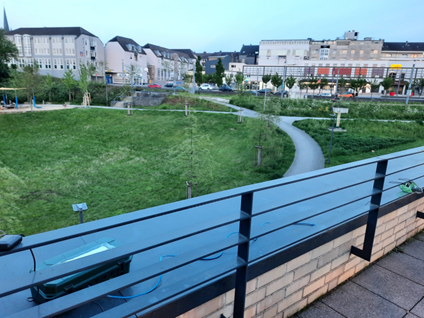
\includegraphics[width=1\linewidth]{bilder/wohnheim_01.png}
    \caption{Bild vom Versuchsaufbau und der Umgebung}
    \label{fig:enter-label}
\end{figure}

\begin{figure}
    \centering
    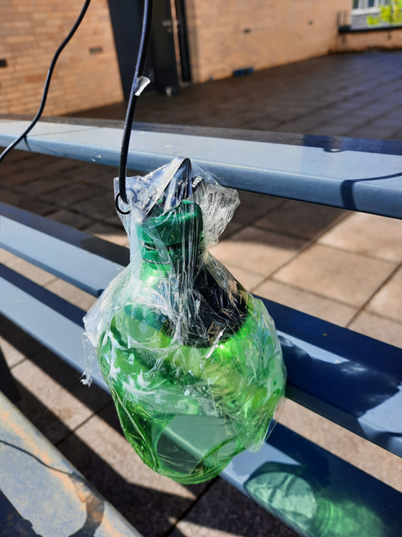
\includegraphics[width=0.5\linewidth]{../grafik.png}
    \caption{Mikrofon in einem Wasserflaschenkopf zum Schutz vor eventuellem Regen}
    \label{fig:enter-label}
\end{figure}

\begin{figure}
    \centering
    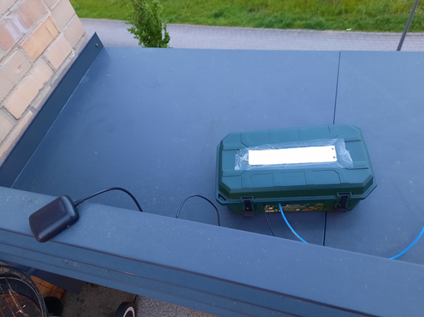
\includegraphics[width=1\linewidth]{../wohnheim_03.png}
    \caption{weiteres Bild vom Versuchsaufbau mit Horchbox und GPS-Tracker}
    \label{fig:enter-label}
\end{figure}

Insgesamt hat dieser ...(26h?) gedauert.
Die einzelnen Testversuche haben ...(12?) Stunden, vier Stunden und zehn Stunden gedauert.

%kurze 

\subsubsection{Testversuch 1.1}

Einstellungen:

Auflistung oder Text oder Bild?

Eckdaten:

Datum: 10.~05.~24
Dauer: 12 h
Ordner: COUNTRIES/Deutschland/Heiligenhaus/Wohnheim\_Dachterrasse\_100524
Koordinaten vom GPS: ja




Da das GPS-Gerät nicht den richtigen Tag bestimmen konnte, liegt das Datumsstempel für die Dateinamen um zwei Tag zurück. Jedoch stimmen die Uhrzeiten, weswegen es für die Validierung der Testergebnisse keine wirklichen Auswirkungen hat.

\subsubsection{Ergebnisse der Analysezeit}

Abbildung .. zeigt einen Ausschnitt der Tabelle mit der berechneten Analysezeit mit der der Jetson 


\begin{figure}
    \centering
    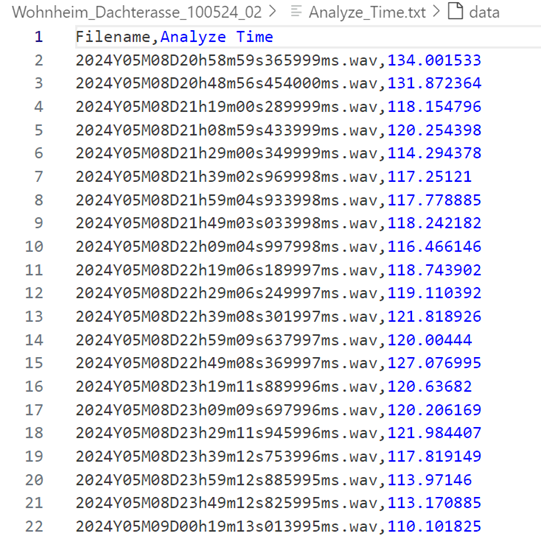
\includegraphics[width=1\linewidth]{bilder/analyze_time_wohnheim.png}
    \caption{Analysezeit des testversuch Nr. 1.1 / Wohnheim Dachterrasse mit overlap von 0}
    \label{fig:enter-label}
\end{figure}

%! da erst nach zwei Audiofiles analysiert wird, sind in den ersten beiden Spalten die files vertauscht. am besten händisch lösen
Die Analysezeit ist hier sogar länger als die Dauer der Audioaufnahme selbst.
Insgesamt hat die Session ... Sekunden gedaurt.

\subsubsection{Testversuch 1.2}

%python3 main110524.py --region COUNTRIES/Deutschland/Heiligenhaus/Wohnheim_Dachterasse_110524.py/ --rtype table --rtype2 audacity --coordinates True --hour 4 --minute 0 --lat 6.968352784 --lon 51.327644614 --trim 10:00 --overlap 1 --min_conf 0.3

Eckdaten:
Datum: 11.~05.~24
%Ordner: COUNTRIES/Deutschland/Heiligenhaus/Wohnheim_Dachterasse_110524
Dauer: 4h 
Koordinaten: True
Dauer pro Audio: 10 Minuten
Overlap: 0
Mindestwahrscheinlichkeit: 0.3


\begin{table}[]
\centering
\caption{Testversuch 1.2}
\label{tab:testversuch1_2}
\begin{tabular}{ll}
Datum                     & 11.05.24                                                                                                                           \\
Ordner                    & \begin{tabular}[c]{@{}l@{}}COUNTRIES/Deutschland/Heiligenhaus/\\ Wohnheim\_Dachterrasse\_110524\end{tabular}                       \\
Dauer                     & 4 h                                                                                                                                \\
Koordinaten               & \begin{tabular}[c]{@{}l@{}}--lon: 51.327644614\\ --lat: 6.96835278\\ --coordinates True\\ Koordinaten wurden gefunden\end{tabular} \\
Dauer pro Audio           & 10:00                                                                                                                              \\
Overlap                   & 0 (default)                                                                                                                        \\
Mindestwahrscheinlichkeit & 0.1 (default)                                                                                                                     
\end{tabular}
\end{table}



\begin{table}[]
\centering
\caption{Testversuch 1.2}
\label{tab:testversuch1_2}
\begin{tabular}{ll}
Datum                     & 11.05.24      \\
Ordner      & \begin{tabular}[c]{@{}l@{}}COUNTRIES/Deutschland/Heiligenhaus/\\ Wohnheim\_Dachterrasse\_110524\end{tabular}                       \\
Dauer                     & 4,0 Stunden\\
Koordinaten & \begin{tabular}[c]{@{}l@{}}--lon: 51.327644614\\ --lat: 6.96835278\\ --coordinates True\\ Koordinaten wurden gefunden\end{tabular} \\
Dauer pro Audio           & 10:00         \\
Overlap                   & 0 (default)   \\
Mindestwahrscheinlichkeit & 0.1 (default)
\end{tabular}
\end{table}


\begin{table}[]
\centering
\caption{Testversuch 1.2}
\label{tab:testversuch1_2}
\begin{tabular}{|l|l|}
\hline
Datum                     & 11.05.24      \\ \hline
Ordner      & \begin{tabular}[c]{@{}l@{}}COUNTRIES/Deutschland/Heiligenhaus/\\ Wohnheim\_Dachterrasse\_110524\end{tabular}                       \\ \hline
Dauer                     & 4,0 Stunden\\ \hline
Koordinaten & \begin{tabular}[c]{@{}l@{}}--lon: 51.327644614\\ --lat: 6.96835278\\ --coordinates True\\ Koordinaten wurden gefunden\end{tabular} \\ \hline
Dauer pro Audio           & 10:00         \\ \hline
Overlap                   & 0 (default)   \\ \hline
Mindestwahrscheinlichkeit & 0.1 (default) \\ \hline
\end{tabular}
\end{table}


\subsubsection{Ergebnisse der Analysezeit}
\begin{figure}
    \centering
    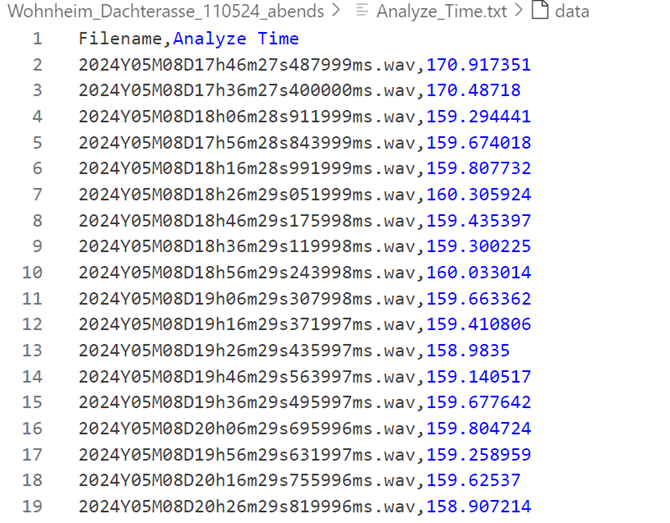
\includegraphics[width=1\linewidth]{bilder/analyze_time_wohnheim_02.png}
    \caption{Enter Caption}
    \label{fig:enter-label}
\end{figure}

\subsubsection{Validierung}


\begin{table}[]
\centering
\caption{11.$\sim$05.$\sim$2024 08:30 Uhr - 8:40 Uhr}
\label{tab:2024Y05M09D08h30m28s201983ms}
\begin{tabular}{|l|l|l|l|l|l|l|}
\hline
Zeitintervall in Sek & Zeitintervall in mm:ss & BirdNET Vogelart & Confidence & Merlin ID & Ohr (0; 0.5; 1) & Klassifikation \\ \hline
63.0  & 01:03 & Tree Pipit        & 0.6763 & -                 & 1 & :| \\ \hline
447.0 & 07:27 & Common Swift      & 0.9929 & -                 & 1 & :| \\ \hline
465.0 & 07:45 & Common Swift      & 0.7170 & European Robin    & 1 & :| \\ \hline
474.0 & 07:54 & Common Chiffchaff & 0.7823 & Common Chiffchaff & 1 & :) \\ \hline
498.0 & 08:18 & Common Chiffchaff & 0.6213 & Common Chiffchaff & 1 & :) \\ \hline
507.0 & 08:27 & Common Chiffchaff & 0.5170 & Common Chiffchaff & 1 & :) \\ \hline
525.0 & 08:45 & Common Chiffchaff & 0.8636 & Common Chiffchaff & 1 & :) \\ \hline
537.0 & 08:57 & Common Chiffchaff & 0.8070 & Common Chiffchaff & 1 & :) \\ \hline
\end{tabular}
\end{table}




\subsection{Testversuch 2  - Balkon in Unterilp}


%Beschreibung des Versuchsaufbau:
Abdeckung zum Schutz vor Wärmeeinstrahlung
Mikrofon hängt über Geländer, um möglichst ohne Schallwände drumherum die Umgebung klar aufnehmen zu können
\begin{figure}
    \centering
    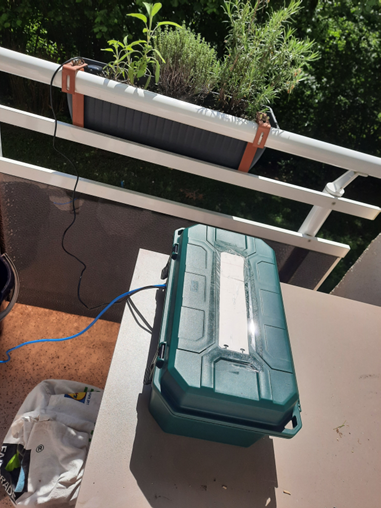
\includegraphics[width=1\linewidth]{bilder/balkon_01.png}
    \caption{Ablageort der Box: Tisch auf dem Balkon}
    \label{fig:enter-label}
\end{figure}

\begin{figure}
    \centering
    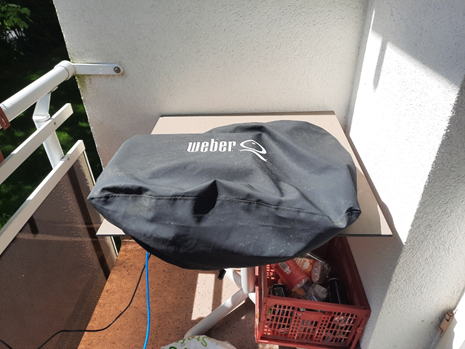
\includegraphics[width=1\linewidth]{bilder/balkon_02.png}
    \caption{Plane als Sonnenschutz über die Box gelegt}
    \label{fig:enter-label}
\end{figure}

\begin{figure}
    \centering
    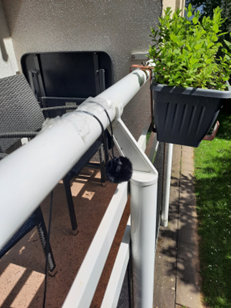
\includegraphics[width=1\linewidth]{bilder/balkon_03.png}
    \caption{Mikrofon hängt über das Balkongeländer, ist mit Tesafilm am Kabel fixiert}
    \label{fig:enter-label}
\end{figure}

\begin{figure}
    \centering
    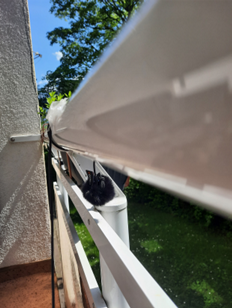
\includegraphics[width=1\linewidth]{bilder/balkon_04.png}
    \caption{weiteres Bild vom Mirkofon aus einem anderen Blickwinkel}
    \label{fig:enter-label}
\end{figure}


\subsubsection{Ergebnisse der Analysezeit}


\begin{figure}
    \centering
    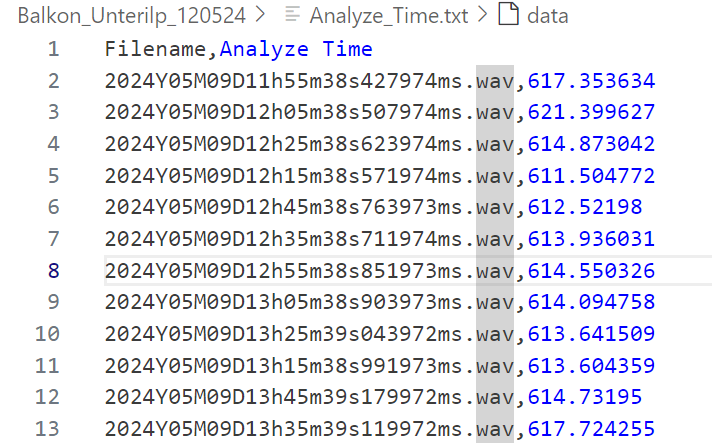
\includegraphics[width=1\linewidth]{bilder/analyze_time_balkon.png}
    \caption{Analysezeit des Testversuch Nr. 2 / Balkon Unterilp mit einem overlap von 2.5}
    \label{fig:analyze_time_balkon}
\end{figure}


\subsection{Start der Software}

-> Vorbereitung z.B. species-list anlegen
-> Verbindung mit dem Jetson aufbauen
-> Befehl an den Jetson schicken


\subsection{}

vierundzwanzig Stunden später:

Was sind die Ergebnisse?





  % Abschnitt 6: Zusammenfassung
  
  \clearpage
  \section{Zusammenfassung und Ausblick%
         \label{sec:zusammen}}

Die Zusammenfassung und der Ausblick schließen den Hauptteil der Ausarbeitung ab. 
Im Gegensatz zur einleitenden Übersicht sollte eine Zusammenfassung losgelöst
von der tatsächlichen Gliederung der Arbeit verfasst sein und sich ganz auf die
Zusammenfassung der Ergebnisse bzw.\ der im Rahmen der Dokumentation
geschriebenen Inhalte beziehen. 

Nach der Zusammenfasung erfolgt ein Ausblick. 
Dieser umfasst zum einen Themen, die im Rahmen der Beschränkungen der
vorliegenden Arbeit nicht abschließend untersucht werden konnten,
zum anderen die Anregung, neue Themen zu untersuchen, die sich im Verlauf der
Bearbeitung als interessant herausgestellt haben. 




Abstract: diese Projekt kann als Biodiversitätserfassungsinstrument dienen und ist ein Hilfsmittel für naturschutz, Schutz der Artenvielfalt und Sammlung von Informationen über das Weltgeschehen.  



Biodiversitätserfassungsinstrument

Bedeutung des Projektes: Naturschutz, Schutz der Artenvielfalt, Informationen über das Weltgeschehen sammeln


%  % Abbildungsverzeichnis
%  \clearpage
%  \listoffigures

  % Literaturverzeichnis
  \clearpage
  % manuell in Inhaltsverzeichnis aufnehmen
  \addcontentsline{toc}{section}{Literatur- und Quellenverzeichnis}
%  \addcontentsline{toc}{section}{References}
  % Umbenennen
  \renewcommand\refname{Literatur- und Quellenverzeichnis} % für deutsche Berichte
  % Literaturverzeichnis anzeigen
  \bibliography{bibliography}
\clearpage

% 
%. Ggf. Bilderverzeichnis
\addcontentsline{toc}{section}{Abbildungsverzeichnis}
\listoffigures
\clearpage

%. Ggf. Tabellenverzeichnis
\addcontentsline{toc}{section}{Tabellenverzeichnis}
\listoftables
\clearpage

%. Ggf. Abkürzungsverzeichnis
% Steht schon vorne.....

%. Ggf. Stichwortverzeichnis
% Stichwortverzeichnis soll im Inhaltsverzeichnis auftauchen
%\addcontentsline{toc}{section}{Stichwortverzeichnis} % für deutsche Berichte
%\addcontentsline{toc}{section}{Index}	% für englische Berichte
% Stichwortverzeichnis endgueltig anzeigen
%\printindex
%\clearpage


 %%%%%%%%%%%%%%%%%%%%%%%%%%%%%%%%%%%%%%%%%%%%%
  % Anhang
  \clearpage
  \appendix
  \addcontentsline{toc}{section}{Anhang} % Für deutsche Berichte 
%  \addcontentsline{toc}{section}{Appendix}	% für englische Berichte 
  % Formatierung des Anhangs
  % Bildnummern aus Nummer des Abschnitts und laufender Nummer zusammensetzen
  %
  % Bei Verwendung eines Bericht-Formats (s.o.) geschieht dies
  % automatisch mit der Kapitelnummer (\chapter – eine Ebene oberhalb
  % von \section). Für das Artikel-Format machen wir es hier manuell.
  %
  \renewcommand{\thefigure}{\Alph{section}.\arabic{figure}}
  \makeatletter\@addtoreset{figure}{section}\makeatother
  % Gleichungsnummern aus Nummer des Abschnitts und laufender Nummer zusammensetzen
  \renewcommand{\theequation}{\Alph{section}.\arabic{equation}}
  \makeatletter\@addtoreset{equation}{section}\makeatother
  % Tabellennummern aus Nummer des Abschnitts und laufender Nummer zusammensetzen
  \renewcommand{\thetable}{\Alph{section}.\arabic{table}}
  \makeatletter\@addtoreset{table}{section}\makeatother
  %%%%
  % Inhalt des Anhangs
  \input{inhalt/anhang}

  % Eidesstattliche Erklärung
  \clearpage
  \fancyhead[L]{Eidesstattliche Erklärung} % Kopfzeile links
  %\addcontentsline{toc}{section}{Eidesstattliche Erklärung}
  %%%%%%%%%%%%%%%%%%%
\section*{Eidesstattliche Erklärung}
%
Ich versichere, dass ich die Arbeit selbständig verfasst und keinen als die angegebenen Quellen und Hilfsmittel benutzt sowie Zitate kenntlich gemacht habe. 
%
\bigskip 

Die Regelungen der geltenden Prüfungsordnung zu Versäumnis, Rücktritt, Täuschung und Ordnungsverstoß habe ich zur Kenntnis genommen. 
%
\bigskip

Diese Arbeit hat in gleicher oder ähnlicher Form keiner Prüfungsbehörde vorgelegen. 
%
\bigskip 

%Ich versichere, die von mir vorgelegte Arbeit selbstständig verfasst zu haben.
%Alle Stellen, die wörtlich oder sinngemäß aus veröffentlichten oder nicht veröffentlichten 
%Arbeiten anderer entnommen sind, 
%habe ich als entnommen kenntlich gemacht. 
%Sämtliche Quellen und Hilfsmittel, die ich für die Arbeit benutzt habe, sind angegeben. 
%Die Arbeit hat mit gleichem Inhalt bzw. in wesentlichen Teilen noch keiner anderen Prüfungsbehörde vorgelegen.
%

\vspace{3cm}
Heiligenhaus, den 
\underline{\hspace*{3cm}}
\hfill 
\begin{tabular}[t]{@{}l@{}}\hline
\hspace*{2.5cm}Unterschrift\hspace*{2.5cm}
\end{tabular}


\end{document}
